\chapter{Konwolucyjne sieci neuronowe}
\label{CNNs}
\textit{Konwolucyjne sieci neuronowe} (ang. \textit{Convolutional Neural Networks}, CNN) są biologicznie inspirowanymi sztucznymi sieciami neuronowymi. Należą do zbioru \textit{głębokich sieci neuronowych} (ang. \textit{Deep Neural Networks}, DNN), które z kolei są podzbiorem \textit{systemów uczących się} (ang. \textit{Machine Learning Systems}) tj. algorytmów nie wymagających explicite programowania do ustalenia swoich parametrów. Algorytmy te często określane są obecnie wspomnianym we wstępie tej rozprawy terminem Wąskiej Sztucznej Inteligencji.

Pierwsze matematyczne formalizmy dotyczące CNN zostały zaproponowane już w latach 40-tych XX wieku, natomiast fundamentalne inspiracje biologiczne dały badania nad korą wzrokową kotów Hubel'a i Wiesel’a z lat 50-tych i 60-tych (zob. \cite{Wurtz2009}). M.in. dzięki pracom tych neurofizjologów ustalono, że kora wzrokowa zawiera złożone układy komórek, które odpowiadają za przetwarzanie informacji z wybranych regionów pola widzenia, sumarycznie pokrywając je w całości. Komórki kory wzrokowej działają zatem jak lokalne filtry przestrzeni wejściowej zaprojektowane tak, aby wydobyć istotne informacje z naturalnych obrazów. Dla przykładu reagują one na orientację linii, kształty i kolory.

W odróżnieniu od naturalnych struktur biologicznych sieci konwolucyjne operują przeważnie na reprezentacji cyfrowej obrazu. Zapisywana jest ona w postaci tablicy liczb tzw. \textit{macierzy} o współrzędnych ($x$, $y$), gdzie $x$ to kolumna macierzy, a $y$ wiersz. W przypadku obrazów trójwymiarowych dochodzi jeszcze trzecia składowa, a zamiast macierzy użyta jest wówczas ogólna postać odwzorowania wieloliniowego, czyli \textit{tensor}.

W obrazach cyfrowych dla każdego punktu ($x$, $y$), tzw. \textit{piksela}, kodowana jest informacja o wartości funkcji obrazowej $I$($x$, $y$). Na tej podstawie dzielimy obrazy na:
\begin{itemize}
	\item binarne – gdzie kodowane są jedynie dwie możliwe wartości $I$ (0 lub 1);
	\item monochromatyczne – gdzie kodowana jest informacja o natężeniu jednej barwy (najczęściej są to odcienie szarości lub brązu tzw. \textit{sepia});
	\item kolorowe – gdzie kodowane są wartości natężenia składowych koloru.
\end{itemize}
Do zakodowania informacji o wartości funkcji $I$ w obrazie binarnym potrzebny jest jeden bit na punkt. Odcienie obrazu monochromatycznego lub pojedyncze składowe punktu obrazu kolorowego kodowane są przy pomocy 8--16 bitów, co uzależnione jest od zakresu wartości występujących w danych lub precyzji wymaganej do obliczeń. Przykładowo, obrazy medyczne przetwarzane w tej pracy należą do grupy obrazów monochromatycznych i są zapisywane w reprezentacji 16 bitowej z uwagi na zakres wartości występujących w sygnale RM.

W sieciach konwolucyjnych, procesy zachodzące w korze wzrokowej są modelowane przy użyciu odpowiednio dobranych parametrów i funkcji służących do ekstrakcji istotnych informacji obrazowych i ich przetwarzania. Parametry wykorzystywane do wstępnej ekstrakcji informacji grupowane są w \textit{filtry}, które realizują funkcję \textit{splotu} maski $K$ z kolejnymi fragmentami funkcji $I$. $K$ jest najczęściej macierzą kwadratową o wymiarze $N$, gdzie zazwyczaj $N$ = {1, 3, 5, 7, 9, 11}. Większe wymiary $K$ nie są często stosowane z uwagi na rosnącą wraz z $N$ złożonością obliczeniową. Równanie splotu dyskretnego można zapisać następująco:
\begin{equation}
	I'\left(x, y\right) = \sum_{j=-n}^{n} \sum_{i=-k}^{k} I\left(x - j, y - i \right)K\left(j, i\right),
\end{equation}
gdzie $I'$ jest nową funkcją obrazową powstałą po filtracji, a $i$ i $j$ to kolejne współrzędne maski filtru w odniesienia do jego punktu centralnego. Dla wartości brzegowych podczas realizacji splotu współrzędne poza sygnałem przyjmują z reguły wartość 0. Rzadziej stosuje się inne metody takie jak: odbicie wartości $I$ obrazu poza jego granicami; powtórzenie wartości $I$ obrazu bez odbicia; modyfikację wymiaru maski filtru na brzegu obrazu, tak by nie wychodziła poza jego granicę.

W kontekście sieci konwolucyjnych, pojedynczy splot filtru z obrazem wejściowym nazywany jest \textit{cechą} (zob. \cite{Hijazi2015}). W ostatnich latach powstało wiele algorytmów do wizualizacji cech umożliwiających wydajną analizę wyników działania sieci konwolucyjnych np.: Saliency Maps \cite{DBLP:journals/corr/SimonyanVZ13}, GradCam \cite{DBLP:journals/corr/SelvarajuDVCPB16} czy CNNVIS \cite{DBLP:journals/corr/LiuSLLZL16}. Zasada działania tych algorytmów bazuje na wstecznej propagacji informacji, co skutkuje możliwością selekcji cech, które mają zasadniczy wpływ na wynik końcowy wnioskowania. Grupy cech obliczane na tym samym obszarze obrazu wejściowego nazywane są \textit{mapami cech} (ang. \textit{feature maps}). Zazwyczaj mapy cech zawierają hierarchicznie uporządkowaną strukturę składającą się z cech od najniższego do najwyższego poziomu komplikacji (np. od charakterystycznych skupisk pikseli, przez obiekty składowe do finalnego kształtu). Do cech najniższego rzędu zaliczyć można:
\begin{itemize}
	\item \textit{krawędzie} -- ciągi punktów o gwałtownych zmianach $I$($x$, $y$);
	\item \textit{rogi} -- przecięcia dwóch krawędzi;
	\item \textit{grzbiety} lub \textit{doliny} -- odpowiednio lokalne maksimum lub minimum funkcji $I$;
	\item \textit{skupiska} (ang. \textit{blobs}) -- obszary jednorodnych wartości funkcji $I$ różniących się znacząco od najbliższego otoczenia; 
	\item \textit{tekstury} -- charakterystyczne, przestrzenne ułożenie wartości funkcji $I$ w powtarzające się wzory.
\end{itemize}

Wszystkie cechy wyższego rzędu są kombinacją wyżej wymienionych składowych podstawowych, tworzących bardziej skomplikowane struktury odpowiadające charakterystycznym obiektom znajdującym się w obrazach wejściowych. 

Na podstawie cech, na końcu toru przetwarzania danych z wykorzystaniem sieci neuronowych, realizowane jest wnioskowanie, gdzie w zależności od problemu można wyszczególnić następujące zadania:
\begin{itemize}
	\item \textit{segmentację} -- podział obrazu na spójne fragmenty, najczęściej wiążące się z wyodrębnieniem \textit{obiektu} $A_1$ z \textit{tła} $A_2$ na podstawie ustalonego progu lub miary np.:
	\begin{equation*}
	\begin{aligned}
	I(x,y) \geq T_p \Rightarrow (x,y) \in A_1 \\
	I(x,y) < T_p \Rightarrow (x,y) \in A_2,
	\end{aligned}
	\end{equation*} 
	przy czym metody ustalania wartości progowej $T_p$ lub wielu wartości {$T_p^1$,...,$T_p^n$} są obszarem szerokich badań (zob. \cite{DBLP:journals/corr/abs-1005-4020});
	\item \textit{klasyfikację} -- przyporządkowanie obiektu do odpowiedniej klasy (np. tkanka zdrowa lub patologiczna);
	\item \textit{detekcję} -- binarne rozróżnienie traktujące o tym czy obiekt znajduje się w obrazie czy nie;
	\item \textit{śledzenie} -- detekcja lub też klasyfikacja obiektów w kolejnych krokach czasowych.
\end{itemize} 

Jeszcze do niedawna tor przetwarzania danych w większości badań wykorzystujących uczenie się maszyn, operacje wyliczenia cech i wnioskowanie końcowego zawierał w dwóch osobnych krokach\footnote{Są wyjątki od tej reguły jak np. \cite{10.1007/978-3-319-58667-0_7}, inkrementalny algorytm SVM.}. Porównanie tego schematu z obecnie funkcjonującym podejściem realizowanym w algorytmach głębokiego uczenia się przedstawiono na Rys. \ref{DLworkflow}.
\begin{figure}[h!]
	\centering
	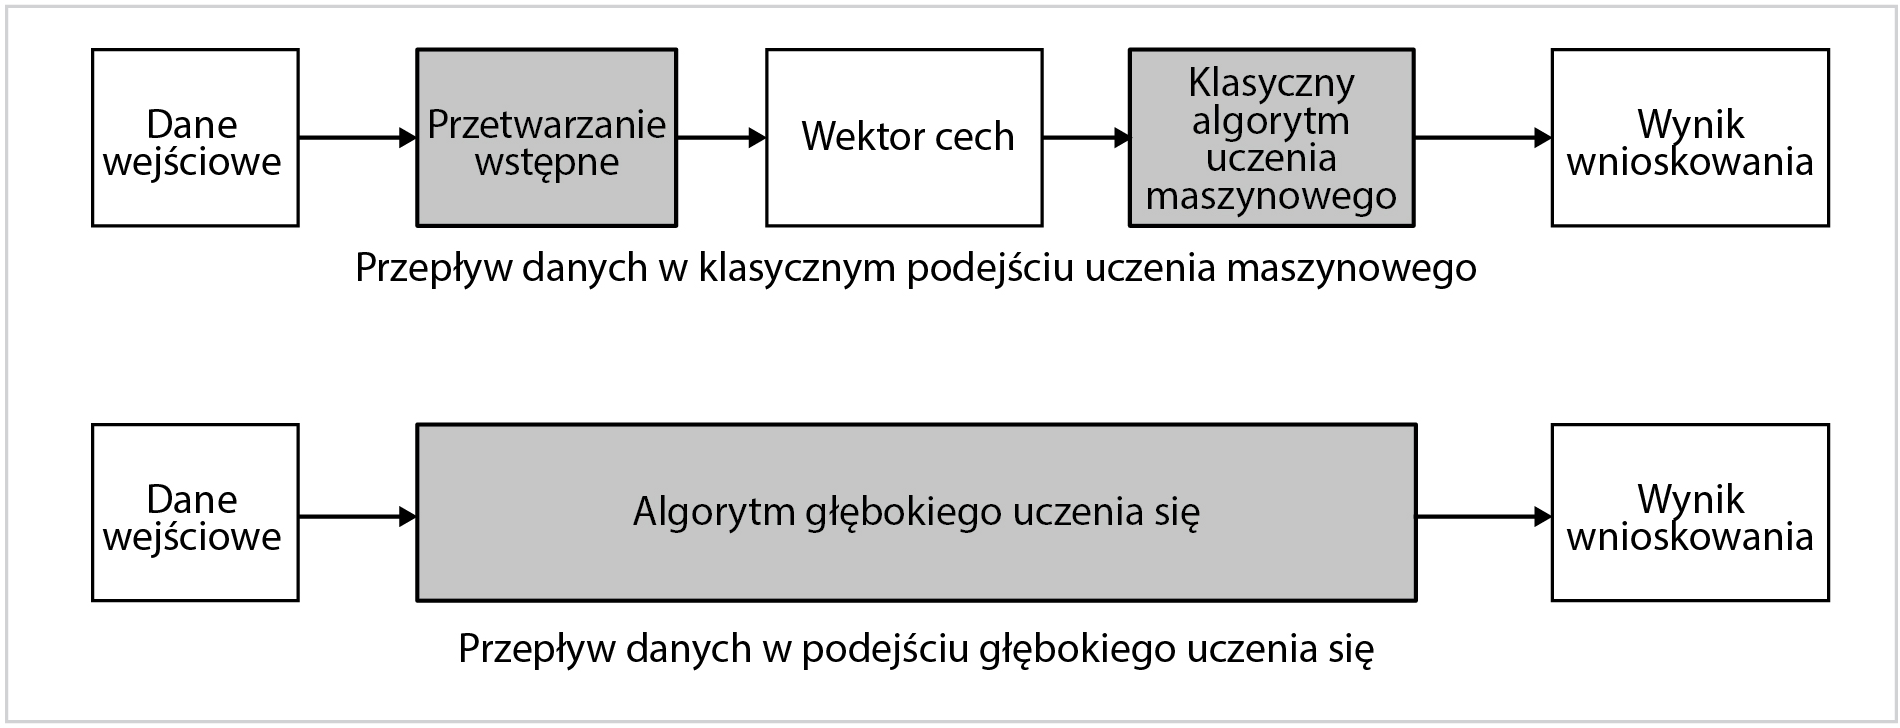
\includegraphics[width=1\textwidth]{figures/DLworkflow.png}
	\caption{Porównanie schematów przetwarzania danych z wykorzystaniem metod głębokiego uczenia się i innych algorytmów.}
	\label{DLworkflow}
\end{figure}

W nowym podejściu zarówno ekstrakcja cech jak i ostateczne wnioskowanie na ich podstawie realizowane jest w jednym kroku, co nazywane jest paradygmatem \textit{end-to-end learning}. Na przestrzeni lat wprowadzano kolejne składowe, które finalnie utworzyły obecnie funkcjonujące podejście. W kontekście poznania tych komponentów, w kolejnej sekcji omówiono dokładniej zarys historyczny przedstawiający ewolucję nowego paradygmatu. 

\section{Rys historyczny}

Pierwszy formalny model neuronu został zaproponowany przez Warrena McCulloch i Waltera Pitts w roku 1943 (zob. \cite{McCulloch1943}). Była to bramka logiczna, której wyjście stawało się aktywne w momencie, gdy liczba aktywnych wejść przekroczyła pewien zdefiniowany próg. Taka zależność sygnału wyjściowego $y$ od sygnałów wejściowych $x_1$,...,$x_n$ została potem nazwana \textit{funkcją aktywacji neuronu}, którą zapisujemy jako:
\begin{equation}
\label{eqActFunc}
y=f\left(x_1, x_2,..., x_n\right)
\end{equation}

W modelu neuronu McCulloch-Pitts można było modyfikować parametr progu, nie istniała natomiast możliwość uczenia się takiej architektury. Problem ten rozwiązano w 1957 proponując sztuczną sieć neuronową zawierającą wiele neuronów z ważonymi połączeniami między sobą (zob. \cite{Rosenblatt1957}). Sieć nazwano perceptronem, co było implikacją zamiłowania jego twórcy Franka Rosenblatta do aplikacji związanych z percepcją, zwłaszcza mowy czy pisma. Schemat sieci pokazano na Rys. \ref{Perceptron}.
\begin{figure}[h!]
	\centering
	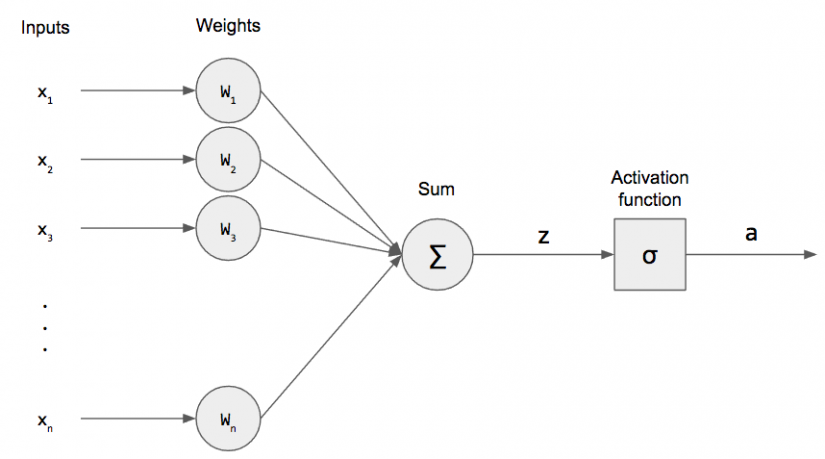
\includegraphics[width=1\textwidth]{figures/perceptron.png}
	\caption{Topologia perceptronu.}
	\label{Perceptron}
\end{figure}

Zastosowanie dodatkowej jednowymiarowej tablicy współczynników, czyli \textit{wektora wag} $w$ = ($w_1$,...,$w_n$) dało możliwość uczenia się poprzez adaptacyjną zmianę wartości poszczególnych jego elementów. W modelu Rosenblatta zastosowano ponadto progową funkcję aktywacji z progiem $T_a$:
\begin{equation}
y(z)=\begin{cases} 0, & n < T_a, \\ 1, & n \ge T_a, \end{cases}
\end{equation}
gdzie $z$ to suma ważona wyjść poszczególnych neuronów:
\begin{equation}
\label{eqLinActFunc}
z=\sum_{i=1}^{n}w_i x_i
\end{equation}

Dla przykładu, w dwuwymiarowej przestrzeni sygnałów wejściowych {$x_1$, $x_2$}  działanie perceptronu można opisać jako wyliczenie funkcji liniowej rozdzielającej obserwacje $o_1$ od $o_2$. W trzech wymiarach będzie to płaszczyzna, a w $n$-wymiarach, hiperpłaszczyzna. Z uwagi na swój liniowy charakter, perceptron proponowany przez Rosenblatta miał wiele ograniczeń, które szczegółowo sformułowali w 1969 roku Marvin Minsky i Seymour Papert w książce \textit{Perceptrons} (zob. \cite{Minsky1969}). Autorzy opublikowali listę problemów, których nie można było rozwiązać z użyciem perceptronu m.in. do najszerzej dyskutowanych należał przykład związany z brakiem możliwości modelowania \textit{funkcji XOR}, aktywującej wyjście przy aktywnym jednym z dwóch wejść.

Część z opisanych przez Minsky-Papert problemów udało się rozwiązać dzięki pracy Davida Rumelharta, Geoffa Hintona i Ronalda Williamsa, którzy opublikowali w 1986 roku pracę \cite{Rumelhart1986}, traktującą o perceptronach wielowarstwowych. Schemat takiej sieci zaprezentowano na Rys. \ref{MLperceptron}
\begin{figure}[h!]
	\centering
	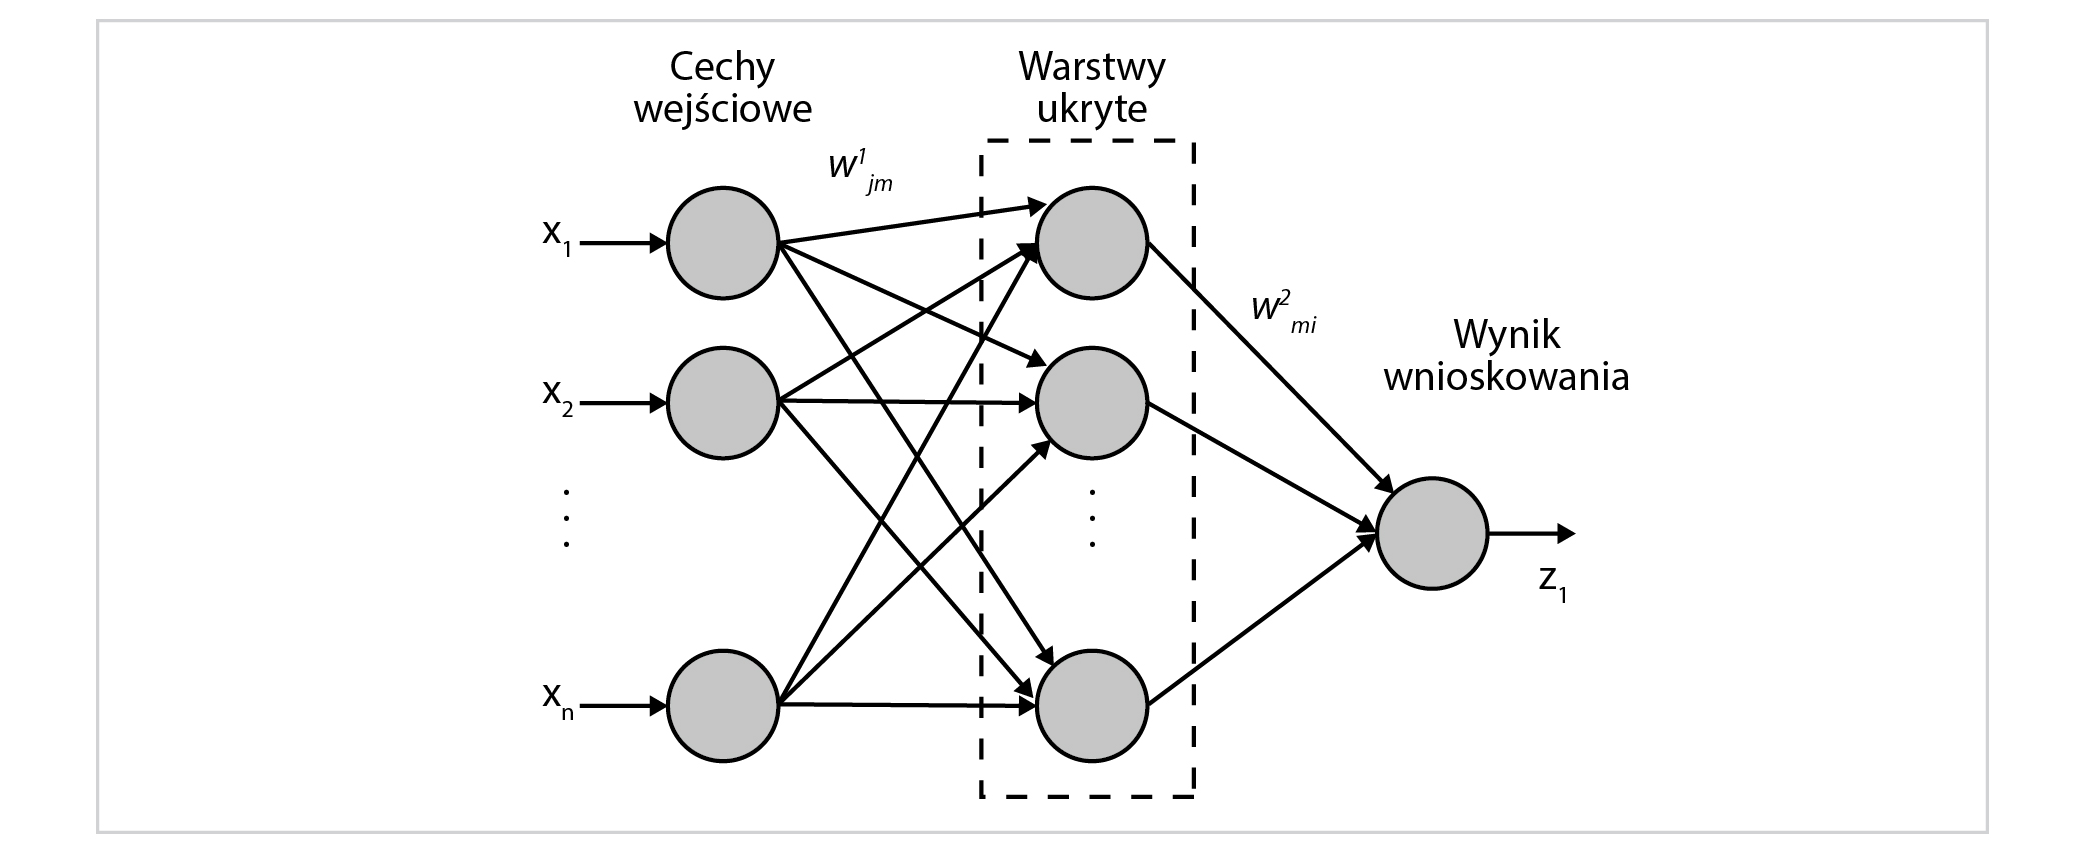
\includegraphics[width=1\textwidth]{figures/MLperceptron.png}
	\caption{Topologia perceptronu wielowarstwowego.}
	\label{MLperceptron}
\end{figure}

Spośród najważniejszych innowacji wprowadzonych w perceptronie wielowarstwowym wyszczególnić można zastosowanie w praktyce nowego algorytmu uczenia się sieci, który został opisany w kolejnej sekcji, jak również wykorzystanie nowej, sigmoidalnej funkcji aktywacji:
\begin{equation}
\label{eqSigActFunc}
y(x) = \frac{1}{1 + e^{-x}}
\end{equation}

Po wprowadzeniu innowacji możliwe stało się modelowanie funkcji XOR jak i innych problemów nieliniowych o praktycznym wymiarze. 

Kolejny przełom nastąpił w 1989 roku kiedy to Yann LeCunn, uczeń Geaoffa Hintona, zaprezentował swoje wyniki klasyfikacji odręcznego pisma z użyciem sieci wielowarstwowych (zob. \cite{NIPS1989_293}). Finalnie, badania te doprowadziły do przedstawienia w 1998 roku protoplasty współczesnych sieci konwolucyjnej -- LeNet (zob. \cite{Lecun1998}). Architekturę LeNet przedstawiono na Rys. \ref{LeNet}.
\begin{figure}[h!]
	\centering
	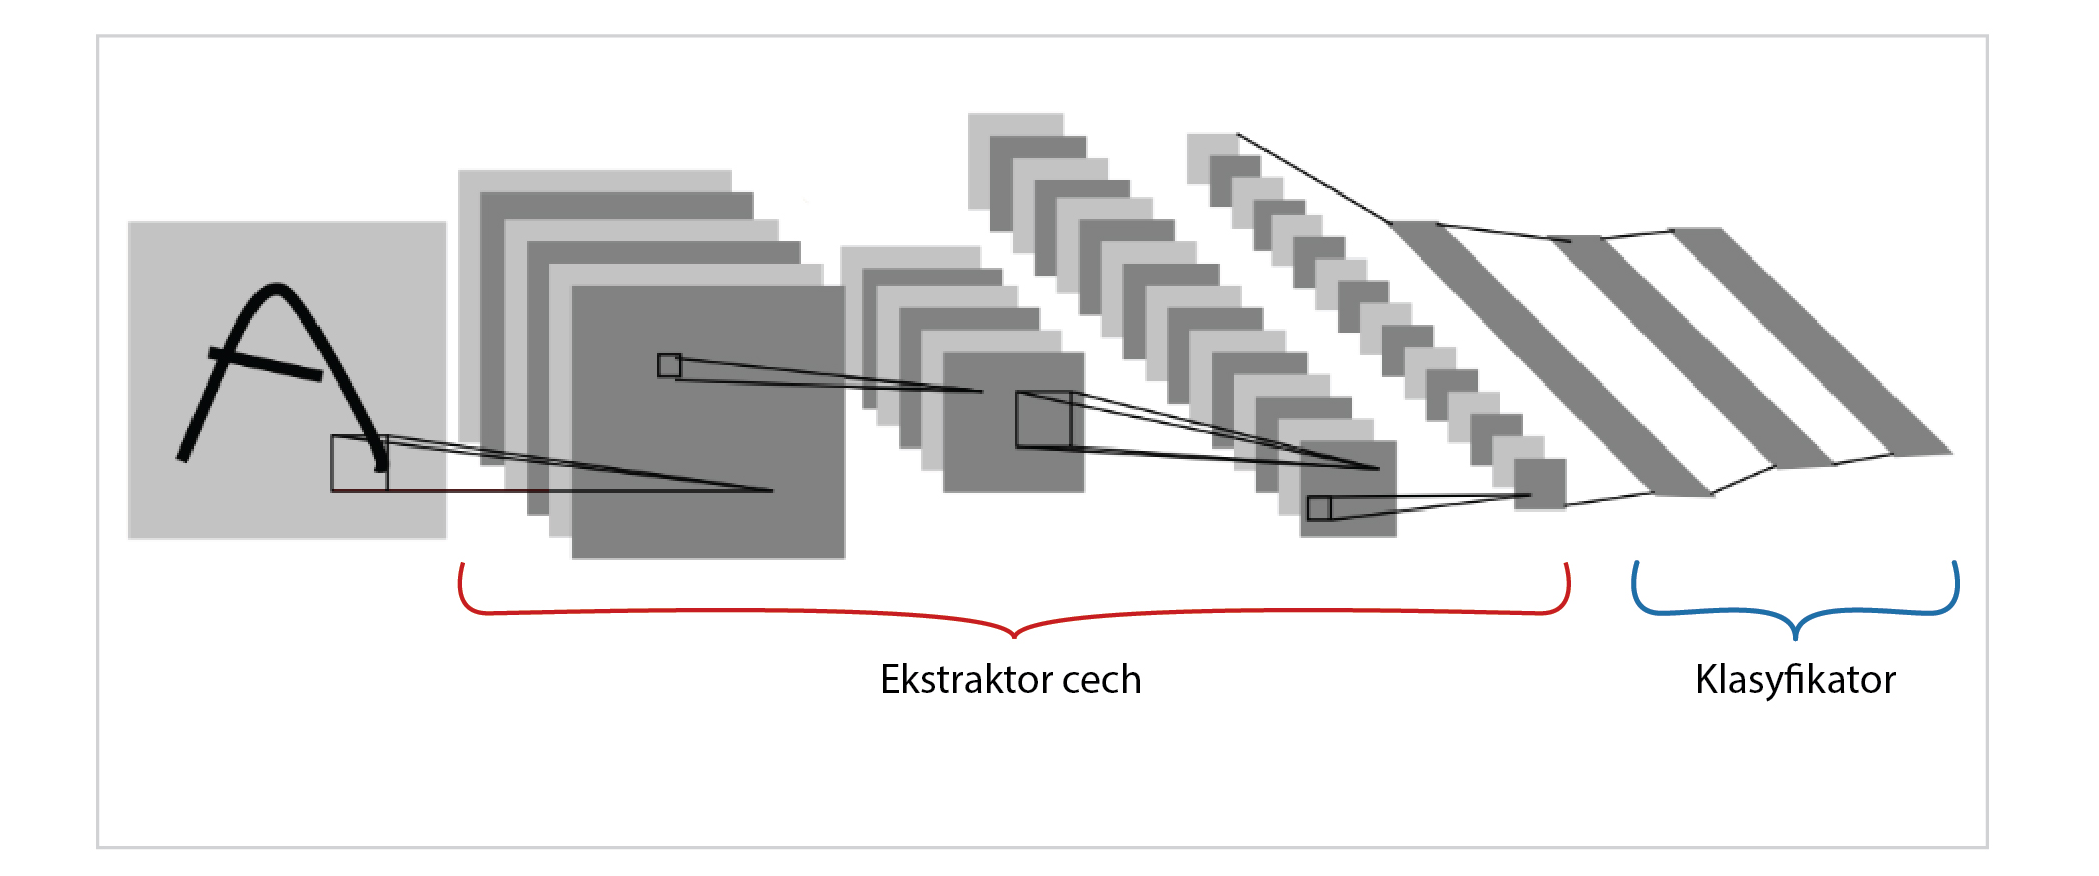
\includegraphics[width=1\textwidth]{figures/lenet.png}
	\caption{Topologia sieci LeNet.}
	\label{LeNet}
\end{figure}

Sieć składa się z 7-miu warstw i zawiera około 60.000 parametrów. Oryginalnie, sygnał wejściowy sieci stanowił obrazek o wymiarach 32$\times$32. W architekturze LeNet zaobserwować można dwie podstawowe składowe współczesnych sieci konwolucyjnych wykorzystywanych do klasyfikacji obrazów tj.:
\begin{itemize}
	\item \textit{ekstraktor cech} -- część służące do automatycznej ekstrakcji wektora cech $w$, zawierająca m.in. filtry.
	\item \textit{klasyfikator} -- część wykorzystywana do zadania wnioskowania końcowego na podstawie $w$.
\end{itemize}  

Przy użyciu takiej architektury możliwe stało się zastosowanie paradygmatu end-to-end learning rozumianego w tym kontekście jako znalezienie w jednym procesie szkolenia się możliwie dobrej transformacji, która surowe obrazy przekształci bezpośrednio w ostateczną klasyfikację. Dokładny opis szkolenia się sieci konwolucyjnych i problemów z tym związanych został przedstawiony w kolejnej sekcji.  

\section{Szkolenie głębokich sieci neuronowych}

Większość algorytmów szkolenia głębokich sieci neuronowych obejmuje zadanie \textit{optymalizacji}, rozumiane jako minimalizację, bądź maksymalizację \textit{funkcji celu} $f$($x$) przez zmianę $x$. W literaturze można też znaleźć inne nazwy funkcji celu takie jak \textit{kryterium}, \textit{funkcja kosztów}, \textit{funkcja strat} lub \textit{funkcja błędów} (por. \cite{Goodfellow-et-al-2016}). 

Podczas zadania optymalizacji bardzo często wykorzystuje się \textit{pochodną funkcji} oznaczaną jako $f'$($x$) lub $\frac{\delta y}{\delta x}$, gdyż niesie ona informacje o nachyleniu funkcji w punkcie $x$. W praktyce funkcje celu są wielowymiarowe dlatego wykorzystywane są \textit{pochodne cząstkowe} informujące o nachyleniu w poszczególnych wymiarach. Wektor zawierający pochodne cząstkowe funkcji nazywany jest \textit{gradientem} i oznaczany jest jako $\bigtriangledown f$($x$). W praktyce wykorzystywane są również: macierz pochodnych cząstkowych tzw. \textit{macierz Jacobiego} oznaczana jako $J$ oraz macierz \textit{drugich pochodnych} cząstkowych (tj. pochodnych pochodnych) tzw. \textit{macierz Hessego} oznaczana jako $H$.

Z uwagi na szybkie znajdowanie lokalnych minimów funkcji celu, to właśnie metody optymalizacji bazujące na wartości gradientu są najczęściej używane w szkoleniu głębokich sieci neuronowych. Inne metody, niegradientowe (zob. \cite{DBLP:journals/corr/TaylorBXSPG16}), przeważnie nie są w tym kontekście wystarczająco efektywne. 

Znalezienie lokalnego minimum nie jest zwykle równoważne z otrzymaniem najlepszego możliwego rozwiązania, jednak w praktyce uznawane jest za satysfakcjonujące. Dla potwierdzenia można przytoczyć następujące fakty wynikające z wielu badań (por. \cite{DBLP:journals/corr/ChoromanskaHMAL14}):
\begin{enumerate}
	\item Dla sieci neuronowych o dużych rozmiarach większość lokalnych minimów charakteryzuje się podobnymi wartościami, przekładającymi się na porównywalny efekt wnioskowania końcowego.
	\item Prawdopodobieństwo znalezienia lokalnego minimum, którego implikacją będą niezadowalające rezultaty wnioskowania przy użyciu sieci maleje wraz ze wzrostem rozmiaru sieci.
	\item Próba znalezienia globalnego minimum bardzo często prowadzi do problemu nadmiernego dopasowania, omówionego dokładniej w sekcji \ref{sec-overffiting}.
\end{enumerate}

Podsumowując, metody gradientowe są wydajne obliczeniowo i prowadzą do znalezienia wielu satysfakcjonujących rozwiązań, które mogą być wykorzystane do rozwiązania praktycznych problemów. 

Zasada działania metod gradientowych bazuje na obieraniu w kolejnych krokach iteracji następujących wartości funkcji $f$, przesuwając się w kierunku spadku gradientu:
\begin{equation}
x' = x - \epsilon \bigtriangledown f(x),
\end{equation} 
gdzie $\epsilon$ to \textit{szybkość uczenia się} -- parametr określający wielkość kroku. 

Funkcja celu w przypadku praktycznych zadań optymalizacyjnych, wykorzystujących głębokie uczenie się jest \textit{funkcją złożoną}, a zatem efekt jej działania jest równoważny operacjom wykonywanym przez kilka lub więcej funkcji po kolei. W takich sytuacjach do obliczeń spadku gradientu wykorzystywane są funkcje, których pochodne są znane.

Aplikuje się je do tzw. \textit{reguły łańcuchowej}. Przypuśćmy, że $v$ = $g$($p$) i $u$ = $f$($g$($p$)) = $f$($v$), gdzie $p$ i $v$ to wektory. Wówczas regułę łańcuchową można zapisać jako:
\begin{equation}
\frac{\delta u}{\delta p_i} = \sum_{j} \frac{\delta u}{\delta v_j} \frac{\delta v_j}{\delta p_i}, 
\end{equation}
co w zapisie wektorowym równoważne jest z równaniem:
\begin{equation}
\label{regLancuch}
\bigtriangledown_x u = (\frac{\delta v}{\delta p})^T \bigtriangledown_q u, 
\end{equation}
gdzie $\frac{\delta v}{\delta p}$ to macierz Jacobiego. 

Regułę łańcuchową zapisaną w \ref{regLancuch} prosto uogólnia się do zmiennych tensorowych (zob. \cite{Goodfellow-et-al-2016}, str. 205) i stosuje się w różnych meta-algorytmach służących do szkolenia sieci. Przykładem jest \textit{algorytm propagacji wstecznej}, który oblicza regułę łańcuchową w wydajnej kolejności stosując działania w grafie takim jak topologia perceptronu wielowarstwowego (zob. \cite{Goodfellow-et-al-2016}).

Proces szkolenia się sieci ma na celu najlepsze możliwe przybliżenie docelowej klasyfikacji bazując na danych przykładach, czyli \textit{zbiorze uczącym} $U$. Algorytmy optymalizacyjne używane do szkolenia głębokich sieci neuronowych zazwyczaj działają pośrednio, optymalizując pewną miarę wydajności $P$, która jest zdefiniowana na \textit{zbiorze testowym}, zawierającym przykłady inne niż w $U$. Często bierze się również pod uwagę dodatkowy podzbiór, rozłączny z $U$ i $T$ -- \textit{zbiór walidacyjny}, który ma pomóc w wyborze najlepszych algorytmów i wartości parametrów wpływających na jakość szkolenia sieci.

W procesie szkolenia zmniejszana jest wartość funkcji kosztów $f$ w oparciu o $U$, a celem jest poprawa $P$. Algorytmy optymalizacyjne wykorzystujące cały zbiór $U$ do liczenia wartości gradientu nazywane są \textit{pakietowymi} lub \textit{deterministycznymi}, gdyż przetwarzają jednocześnie wszystkie przykłady szkoleniowe. Te, które używają jednego przykładu na raz są nazywane \textit{stochastycznymi}. Natomiast w praktyce przy szkoleniu głębokich sieci stosowane są algorytmy \textit{minipakietowe}, wykorzystujące więcej niż jeden przykład, ale mniej niż cały zbiór. Z reguły są to liczby z przedziału 8--256. Takie podejście zapewnia kompromis między szybkością obliczeń a dokładnością estymacji wartości gradientu.

Przykładem algorytmu minipakietowego jest \textit{stochastyczny spadek gradientu} (ang. \textit{stochastic gradient descent}, SGD). Bazuje on na założeniu, że estymację gradientu można otrzymać wyliczając średnią gradientu z minipakietu $m$ przykładów. Kolejne kroki algorytmu można zapisać następująco:
\begin{enumerate}
	\item Wybierz wartość parametru szybkości uczenia się $\epsilon_k$.
	\item Wybierz minipakiet złożony z $m$ przykładów ze zbioru szkoleniowego.
	\item Oblicz estymację gradientu $g$ = $\frac{1}{m}\bigtriangledown \sum_{i=1}^{m}L(x_i, y_i, f)$, gdzie $L$ to funkcja strat dla jednego przykładu o wejściowej wartości próbki $x_i$ i oczekiwanym wyjściu $y_i$.
	\item Zastosuj aktualizację wartości funkcji celu równą $\epsilon_k g$.
	\item Jeżeli kryterium stopu nie zostało spełnione wróć do kroku 2. 
\end{enumerate}

Kryterium stopu jest najczęściej określone liczbą iteracji lub satysfakcjonującą wartością funkcji $f$. Kwestia optymalnego wyboru parametru $\epsilon_k$ zależy od zadanego problemu. Najczęściej stosowane są metody empiryczne, przy czym zazwyczaj $\epsilon_k$ maleje wraz ze zbliżaniem się do satysfakcjonującego rozwiązania.

Parametry algorytmów szkoleniowych nazywane są \textit{hiperparametrami}, gdyż nie są wyznaczane bezpośrednio w procedurze uczenia się. Strategia nadawania hiperparametrom wartości początkowych jest silnie dyskutowana w literaturze (zob. \cite{Koch2017AutomatedHT}) i jej kompleksowy opis wykracza poza zakres tej pracy. Warto jednak wspomnieć o algorytmach z adaptacyjną szybkością uczenia się, gdyż jest to jeden z najtrudniejszych do ustawienia, a jednocześnie bardzo istotny hiperparametr. Do tych algorytmów należą m.in.:
\begin{itemize}
 \item Adaptive Gradient Algorithm (AdaGrad) \cite{Duchi:2011:ASM:1953048.2021068} -- wykorzystywany do indywidualnej adaptacji szybkości uczenia się wszystkich parametrów modelu, skalując je odwrotnie proporcjonalnie do pierwiastka kwadratowego sumy wszystkich historycznych kwadratów gradientów.
 \item Root Mean Square Propagation (RMSProp) \cite{SCHMIDHUBER201585} -- modyfikacja AdaGrad, w której zamiast akumulacji gradientu wykorzystuje się wykładniczo ważoną ruchomą średnią z gradientu.
 \item Adaptive moments algorithm (Adam) \cite{DBLP:journals/corr/KingmaB14} -- W porównaniu z RMSProp, Adam poza momentem pierwszego rzędu (tj. średnią) wykorzystuje również moment drugiego rzędu (tj. \textit{wariancję}). Dokładniej rzecz biorąc, w algorytmie liczona jest wykładnicza ruchoma średnia gradientu i kwadrat z gradientu oraz parametry $\beta_1$ i $\beta_2$, które kontrolują zakres liczenia średnich.
\end{itemize}
W momencie pisania tej pracy, algorytm Adam jest najczęściej rekomendowany jako domyślna metoda szkolenia głębokich sieci neuronowych, dlatego poniżej zamieszczono jego dokładny opis:
\begin{enumerate}
	\item Wybierz wartość początkową $\epsilon$, $\beta_1$, $\beta_2$ oraz ustaw początkowe wartości zmiennych momentu 1 i 2 stopnia $s$ = 0 i $r$ = 0, wartość kroku czasowego $t$ = 0 i stałą $\sigma$ używaną do stabilizacji numerycznej.
	\item Wybierz minipakiet złożony z $m$ przykładów ze zbioru szkoleniowego.
	\item Oblicz estymację gradientu $g$ = $\frac{1}{m}\bigtriangledown \sum_{i=1}^{m}L(x_i, y_i, f)$ i zwiększ $t$ o 1.
	\item Aktualizuj estymację pierwszego momentu. $s$ $\mapsto$ $\beta_1$$s$ + (1-$\beta_1$)$g$.
	\item Aktualizuj estymację drugiego momentu. $r$ $\mapsto$ $\beta_2$$r$ + (1-$\beta_2$)$g\bigodot g$, gdzie $\bigodot$ to iloczyn skalarny dwóch gradientów.
	\item Skoryguj obciążenie momentu pierwszego rzędu $s$ = $\frac{s}{1-\beta_1^t}$.
	\item Skoryguj obciążenie momentu drugiego rzędu $r$ = $\frac{r}{1-\beta_2^t}$.
	\item Zastosuj aktualizację wartości funkcji celu równą -$\epsilon$$\frac{s}{\sqrt{r}+\sigma}$.
	\item Jeżeli kryterium stopu nie zostało spełnione wróć do kroku 2. 
\end{enumerate}

Ocena procesu szkolenia się sieci polega na obliczeniu odpowiednich miar i współczynników odzwierciedlających przybliżenie zbioru $T$ albo $W$ przez znalezione rozwiązanie. W powszechnym problemie klasyfikacji binarnej, występującym również w tej pracy, w kontekście oceny efektywności algorytmów można wyszczególnić opisane poniżej parametry i miary.

Parametry:
\begin{itemize}
	\item \textit{Fałszywie dodatnia klasyfikacja} (\textit{FP} od ang. \textit{False Positive}) -- liczba obserwacji zaklasyfikowanych jako pozytywne, a należących do klasy obserwacji negatywnych.
	\item \textit{Fałszywie ujemna klasyfikacja} (\textit{FN} od ang. \textit{False Negative}) -- liczba obserwacji zaklasyfikowanych jako negatywne, a należących do klasy obserwacji pozytywnych. 
	\item \textit{Prawdziwie pozytywna klasyfikacja} (\textit{TP} od ang. \textit{True Positive}) -- liczba wyników poprawnie zaklasyfikowanych jako pozytywne. 
	\item \textit{Prawdziwie negatywna klasyfikacja} (\textit{TN} od ang. \textit{True Negative}) -- liczba wyników poprawnie zaklasyfikowanych jako negatywne.
\end{itemize}

Miary:
\begin{itemize}
	\item \textit{Dokładność klasyfikacji} (ang. \textit{Accuracy}) -- $ACC = \frac{TP + TN}{TP+TN+FP+FN}$.
	\item \textit{Czułość klasyfikacji} (ang. \textit{Sensitivity}) -- $TPR = \frac{TP}{TP + FN}$.
	\item \textit{Swoistość klasyfikacji} (ang. \textit{Specificity}) -- $TNR = \frac{TN}{TN + FP}$.
	\item \textit{Wartość predykcyjna dodatnia} (ang. \textit{Precision}) -- $PPV = \frac{TP}{TP + FP}$.
	\item \textit{Wartość predykcyjna ujemna} (ang. \textit{Negative precision}) -- $NPV = \frac{TN}{TN + FN}$.
\end{itemize}

W problemach empirycznych dąży się do maksymalizowania TP, TN, ACC, TPR, TNR, PPV i NPV oraz minimalizowania FP i FN. Prawidłowe podejście polega również na wybraniu możliwie efektywnej architektury sieci. Problemy z tym związane zostaną omówione w kolejnych podsekcjach.

\subsection{Problem nadmiernego dopasowania}
\label{sec-overffiting}

Dążenie do najlepszego możliwego przybliżenia zbioru $U$ wprowadza niepożądane zjawisko zwane \textit{nadmiernym dopasowaniem}. Wtedy to dokładność klasyfikacji zbioru $U$ jest wysoka lub nawet bezbłędna, natomiast znacznie niższa jest dokładność klasyfikacji zbioru testowego $T$ i walidacyjnego $W$. W praktyce oznacza to, że model staje się mało użyteczny, gdyż wnioskowanie na nowych danych charakteryzuje się niską dokładnością.

Zatem ogólnym dążeniem w procesie szkolenia się sieci jest osiągnięcie \textit{maksymalnej generalizacji} klasyfikacji. Sieć o wysokim współczynniku generalizacji lepiej klasyfikuje ogół zadanych wektorów wejściowych niż sieć, która ma niski współczynnik generalizacji i jest nadmiernie dopasowana do zbioru $U$. Właściwym działaniem jest ustalenie maksymalnie ogólnych, dostatecznych warunków poprawnej klasyfikacji, dzięki którym wzrasta prawdopodobieństwo, że przykład spoza zbioru $U$ będzie poprawnie klasyfikowany. W tym celu można zastosować \textit{metodę oceny krzyżowej} (ang. \textit{cross-validation}). Metoda ta polega na podziale zbioru uczącego na $s$ segmentów $D$, z których każdy w innej iteracji służy jako zbiór testujący i walidacyjny, a pozostałe segmenty pełnią rolę zbioru uczącego. Podział zobrazowany jest na Rysunku \ref{cross-validation}.
\begin{figure}[h!]
	\centering
	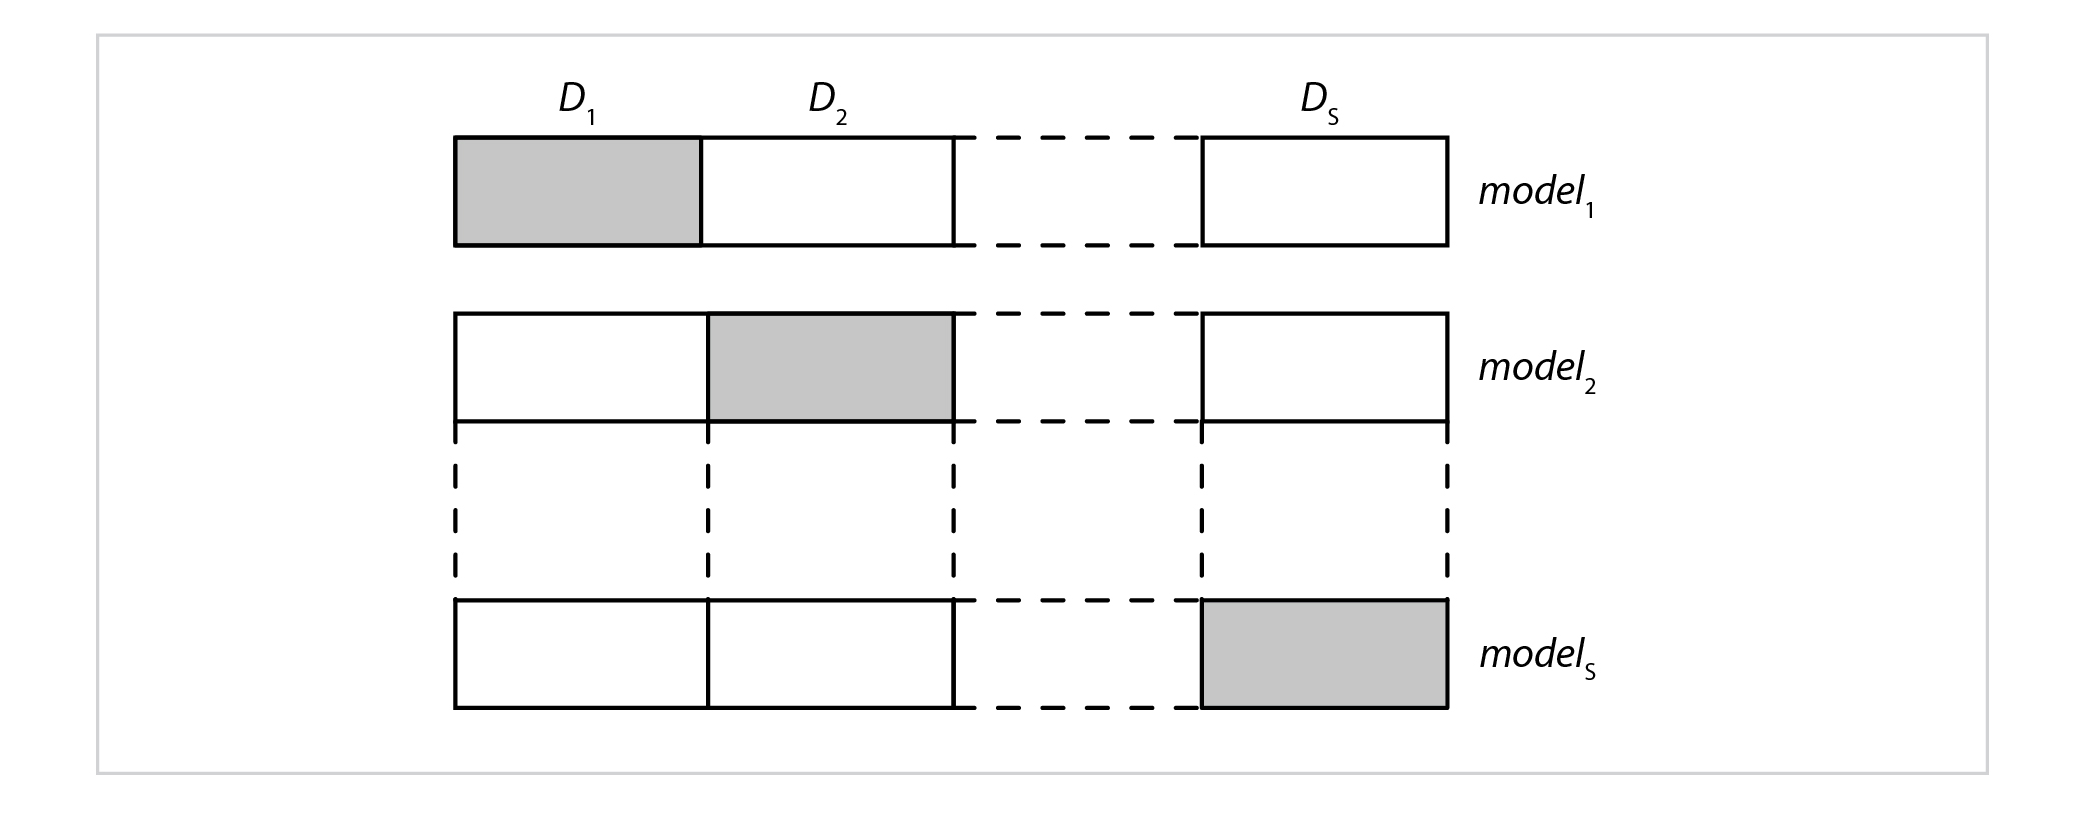
\includegraphics[width=1\textwidth]{figures/cross-validation.png}
	\caption{Reprezentacja graficzna oceny krzyżowej.}
	\label{cross-validation}
\end{figure}
Stosując metodę oceny krzyżowej dla różnych modeli sieci można stwierdzić, który z nich spełnia najlepiej kompromis między dobrą klasyfikacją zbioru $U$ i wysoką generalizacją.

Kombinacja predykcji wielu różnych modeli jest bardzo wydajną metodą stosowaną do polepszenia generalizacji i zmniejszenia błędu klasyfikacji na zbiorach innych niż $U$ (zob. \cite{Bell2007, Breiman2001}). Jednak współczesne sieci neuronowe, których przykłady zostały opisane w dalszych sekcjach, mogą zawierać miliony parametrów i ich optymalizacja jest wymagająca obliczeniowo. Z tego powodu w praktyce ogranicza się liczbę segmentów obierając $s$ $\in$ $\langle$3, 10$\rangle$.

Innym podejściem do zwiększenia generalizacji, zaproponowanym w 2012 w \cite{DBLP:journals/corr/abs-1207-0580}, jest technika \textit{dropout}, której główna idea bazuje na zerowaniu wyjścia neuronów sieci z prawdopodobieństwem 0,5 przy każdej iteracji treningu sieci. Neurony, które są w ten sposób tymczasowo dezaktywowane nie mają wpływu w danej iteracji na predykcję sieci i nie są uwzględniane przy wstecznej propagacji gradientu. Podejście to można porównać do treningu w każdej iteracji różnych modeli sieci. Dla przykładu w \cite{Krizhevsky2012} wykazano, że metoda dropout wymaga jedynie 2 razy więcej iteracji do przybliżenia zbioru $U$, przy czym uzyskuje znacznie lepszą generalizację. 

Kluczowym składnikiem potrzebnym do treningu sieci i maksymalizacji generalizacji jest odpowiedni rozmiar zbioru danych. Jest to problem szeroko dyskutowany, gdyż zwłaszcza w danych medycznych istnieje szereg ograniczeń związanych z dostępem i akwizycją odpowiedniego materiału badawczego (np. ograniczenia prawne, związane z prywatnością lub z etyką). W przypadku, gdy zgromadzenie odpowiedniego zbioru danych jest niemożliwe, pewnym rozwiązaniem problemu jest zastosowanie metod jego sztucznego powiększania (ang. \textit{data augmentation}).

Dla obrazów stosuje się metody \textit{afinicznych przekształceń} zgodne z definicją algebraiczną:
\begin{equation}
	\mathbf o \mapsto \mathbf{Ao} + \mathbf b,
\end{equation}
gdzie $A$ jest macierzą przekształcenia liniowego, a $b$ wektorem przesunięcia. Jako przykłady takich przekształceń dla dwuwymiarowych obrazów można wymienić:
\begin{itemize}
	\item \textit{rotację} -- obrót obrazu o kąt $\theta$, gdzie:
	\begin{equation}
	A = \begin{bmatrix} 
	\cos \theta & \sin \theta\\
	-\sin \theta & \cos \theta
	\end{bmatrix}
	\end{equation}	
	\item \textit{odbicie lustrzane} -- odwrócenie kolejności pikseli w każdym wierszu, gdzie:
	\begin{equation}
		A = \begin{bmatrix} 
		-1 & 0\\
		0 & 1
	\end{bmatrix}
	\end{equation}
	\item \textit{skalowanie} -- zmiana rozmiaru obrazu o $S$, gdzie:
	\begin{equation}
			A = \begin{bmatrix} 
		S_x & 0\\
		0 & S_y
	\end{bmatrix}
	\end{equation}
	\item \textit{translację} -- przesunięcie punktów obrazu o wektor $b$.
\end{itemize}

Analogiczne równania istnieją dla obrazów trójwymiarowych (zob. \cite{Hill06}). W określonych przypadkach używane są również nieafiniczne przekształcenia. Dla przykładu, w \cite{DBLP:journals/corr/RonnebergerFB15} wykorzystano nieliniowe deformacje do powiększenia zbioru 30-tu obrazów mikroskopowych przedstawiających macierz komórkową i uzyskano znacząco lepsze wyniki detekcji komórek od istniejących w 2015 r. najlepszych rozwiązań.

Dla danych medycznych należy szczególnie zwrócić uwagę, aby powiększony zbiór zawierał dane przypominające przypadki występujące w rzeczywistości np. nieduże obroty występujące u pacjentów skanowanych Rezonansem Magnetycznym lub niewielkie skalowania rozmiaru kości widocznych w Tomografii Komputerowej. Szeroka dyskusja prowadzona się również na temat wykorzystania sztucznie generowanych zbiorów danych o czym więcej można przeczytać w \cite{DBLP:journals/corr/SixtWL16, Litjens2017}. 

\subsection{Problem redukcji wymiarowości}
\label{DimReduction}
Duży rozmiar wektora cech prowadzi do problemu nazwanego \textit{przekleństwem wymiarowości} (ang. \textit{curse of dimensionality}). Określenie zostało po raz pierwszy sformułowane przez Richarda Bellmana w latach 50-tych XX wieku. Naukowiec ten podczas swojej pracy obserwował algorytmy doskonale działające w 3 wymiarach, a prezentujące znacząco gorsze wyniki w hiperprzestrzeni (zob. \cite{Bellman:1957}). 

Problem przekleństwa wymiarowości ma dwie główne przyczyny: (1) nie wszystkie cechy są jednakowo znaczące w kontekście rozróżnienia danych; (2) w miarę wzrostu rozmiaru przestrzeni cech, liczba obserwacji w zbiorze uczącym potrzebnych do wiarygodnego oszacowania funkcji wyjściowej rośnie wykładniczo.  

Problem (1) jest szczególnie istotny w dość prostych algorytmach takich jak np. algorytm $K$-najbliższych sąsiadów, gdzie do poprawnego działania należy policzyć dystans pomiędzy sąsiednimi obserwacjami. Uwzględniając dużą liczbę nieistotnych cech jako argumenty funkcji dystansu uzyskuje się wyniki utrudniające lub nawet uniemożliwiające poprawną klasyfikację zbioru. Konieczna jest wówczas adaptacja wpływu poszczególnych cech np. poprzez wprowadzenie wektora wag.

Problem (2) ma duże implikacje w praktyce stosowania sieci neuronowych, gdyż uzyskanie odpowiednio dużego, ustrukturyzowanego zbioru danych stanowi przeważnie wyzwanie. W poprzedniej podsekcji omówiono możliwość sztucznego powiększania zbioru danych. Inną opcją jest zmniejszenie rozmiaru wektora cech, co może być wykonane na dwa sposoby:

\begin{itemize}
\item wybór podzbioru istotnych cech o liczności $n'$ $<<$ $n$,
\item przekształcenie oryginalnych $n$ zmiennych na nowy zbiór $n'$ cech, gdzie ponownie $n'$ $<<$ $n$.
\end{itemize}

W pierwszym przypadku, wybór podzbioru istotnych cech polega na określeniu minimalnego podzbioru, dla którego rozkład prawdopodobieństwa różnych klas obiektów jest jak najbliższy oryginalnemu rozkładowi uzyskanemu z wykorzystaniem wszystkich cech. Do tych zagadnień wykorzystywane są metody takie jak:
\begin{itemize}
	\item \textit{miary siły związku} -- określające podobieństwo między rozkładami zmiennych losowych. Najczęściej stosowana jest \textit{korelacja Pearsona}, której współczynnik $r$ dla dwóch zmiennych losowych $X1$ i $X2$ zapisywany jest następującym wzorem:
	\begin{equation}
	r_{X1X2} = \frac{\sum_{i=1}^n (X1_i - \overline{X1})(X2_i - \overline{X2})}{\sqrt{\sum_{i=1}^n (X1_i - \overline{X1})^2} \sqrt{\sum_{i=1}^n (X2_i - \overline{X2})^2}},
	\end{equation}
	gdzie $X1_i$, $X2_i$ to wartości kolejnych obserwacji, a $\overline{X1}$ i $\overline{X2}$ to ich średnie. Innymi słowy tak zapisany współczynnik $r_{X1X2}$ jest ilorazem \textit{kowariancji} i iloczynu \textit{odchyleń standardowych} zmiennych $X1$ i $X2$.
	\item \textit{miary entropii względnej} --  określające rozbieżności między rozkładami zmiennych losowych. Najczęściej stosowana jest \textit{dywergencja Kullbacka-Leiblera}, której współczynnik $d_{KL}$ dla dwóch rozkładów prawdopodobieństwa $p_k$ i $q_k$ zapisany jest wzorem: 
	\begin{equation}
	d_{KL}(p_k, q_k) = \sum_{i} p_k(i) \log_2 \frac{p_k(i)}{q_k(i)}
	\end{equation}
	\item \textit{teoria zbiorów przybliżonych} -- wykorzystująca informacje o elementach zbioru i klasyczną teorię zbiorów do porównywania rozkładów (zob. \cite{Kowalik2003}).
\end{itemize}
Podobieństwo rozkładów ocenione na podstawie powyższych miar daje możliwość skutecznej redukcji wymiarowości z zachowaniem efektywności algorytmu.

W celu selekcji cech można również stosować różnego rodzaju, specjalnie zaprojektowane regresje. Do najbardziej powszechnie stosowanych należą algorytmy regresji grzbietowej, LASSO (od ang. \textit{Least Absolute Shrinkage and Selection Operator}) oraz Elastic Net. Różnią się one definicją zadania minimalizacji wektora cech $w$:

\begin{equation}
\textrm{Regresja grzbietowa-- } \underset{w}{min} ||X*w-Y||_2^2 + \alpha ||w||_2^2;
\label{equ:ridgeReg}
\end{equation}
\begin{equation}
\textrm{LASSO-- } \underset{w}{min} ||X*w-Y||_2^2 + \alpha ||w||_1;
\label{equ:lassoReg}
\end{equation}
\begin{equation}
\textrm{Elastic Net-- } \underset{w}{min} { \frac{1}{2n_{samples}} ||X w - y||_2 ^ 2 + \alpha \rho ||w||_1 + \frac{\alpha(1-\rho)}{2} ||w||_2 ^ 2}.
\label{equ:elasticNet}
\end{equation}

W szczególności istotny jest czynnik regulujący dołączony do klasycznego zadania regresji liniowej będący pierwszym elementem każdego zadania minimalizacji. W regresji grzbietowej dodatkowo dodawany jest warunek minimalizacji \textit{Normy L2} z wektora $w$ ($\left \| w \right \|_2 =\sqrt{ \sum_{k=1}^{n}\left |w_k  \right |^2}$), dzięki czemu wymuszane jest, aby poszczególne współczynniki nie były za duże. W regresji LASSO stosowana jest \textit{Norma L1}, ($\left \| w \right \|_1 = \sum_{k=1}^{n}\left |w_k  \right |$), dzięki czemu preferowane są rozwiązania, w których wektor jest rzadki, co przekłada się na efektywny wybór cech z grup silnie skorelowanych. Regresja Elastic Net łączy w sobie cechy regresji grzbietowej oraz LASSO, poprzez zastosowanie dwóch typów norm jednocześnie, których istotność względem siebie kontroluje parametr $\rho$. Minusem tego podejścia jest większa złożoność obliczeniowa i konieczność doboru wartości dodatkowego parametru. Z uwagi na definicję zadania minimalizacji, powyższe algorytmy znajdują zastosowania głównie w problemach, gdzie występują zależności liniowe. Do nieliniowych problemów stosuje się częściej bardziej skomplikowane algorytmy typu lasy losowe.

W kolejnym omawianym przypadku, tj. gdy zaistnieje potrzeba przekształcenia przestrzeni cech i wyliczenia nowego zbioru, metodą \textit{state-of-the-art} jest algorytm \textit{analizy składowych głównych} (ang. \textit{Principal Component Analysis}, w skr. \textit{PCA}) opracowany przez Karla Pearsona w 1901 r (zob. \cite{PCA}).  

Istotą PCA jest przekształcenie początkowych, skorelowanych cech w nowy zbiór nieskorelowanych zmiennych. Nowe zmienne, tzw. \textit{składowe główne} lub \textit{czynniki główne}, powstają z przekształcenia oryginalnych zmiennych skorelowanych w taki sposób, aby w maksymalnym stopniu wyjaśniać całkowitą wariancję w próbie cech oryginalnych. Wariancje składowych głównych są \textit{wartościami własnymi} macierzy kowariancji oryginalnych zmiennych. Innymi słowy są to \textit{wartości skalarne} (pojedyncze liczby) opisujące poziom wariancji w danych w stosunku do zadanych \textit{ortogonalnych wektorów}, tj. takich, dla których iloczyn skalarny równy jest 0, co w przestrzeni Euklidesowej oznacza, że kąt pomiędzy wektorami równy jest 90$^\circ$.

Dla przykładu, pierwsza składowa główna redukuje największą część zróżnicowania, druga kolejną, której nie redukowała poprzednia itd. Składowych głównych jest zawsze tyle ile wymiarów danych. Przykład dwuwymiarowy został przedstawiony na Rys. \ref{PCA-2dim}.
\begin{figure}[h!]
	\centering
	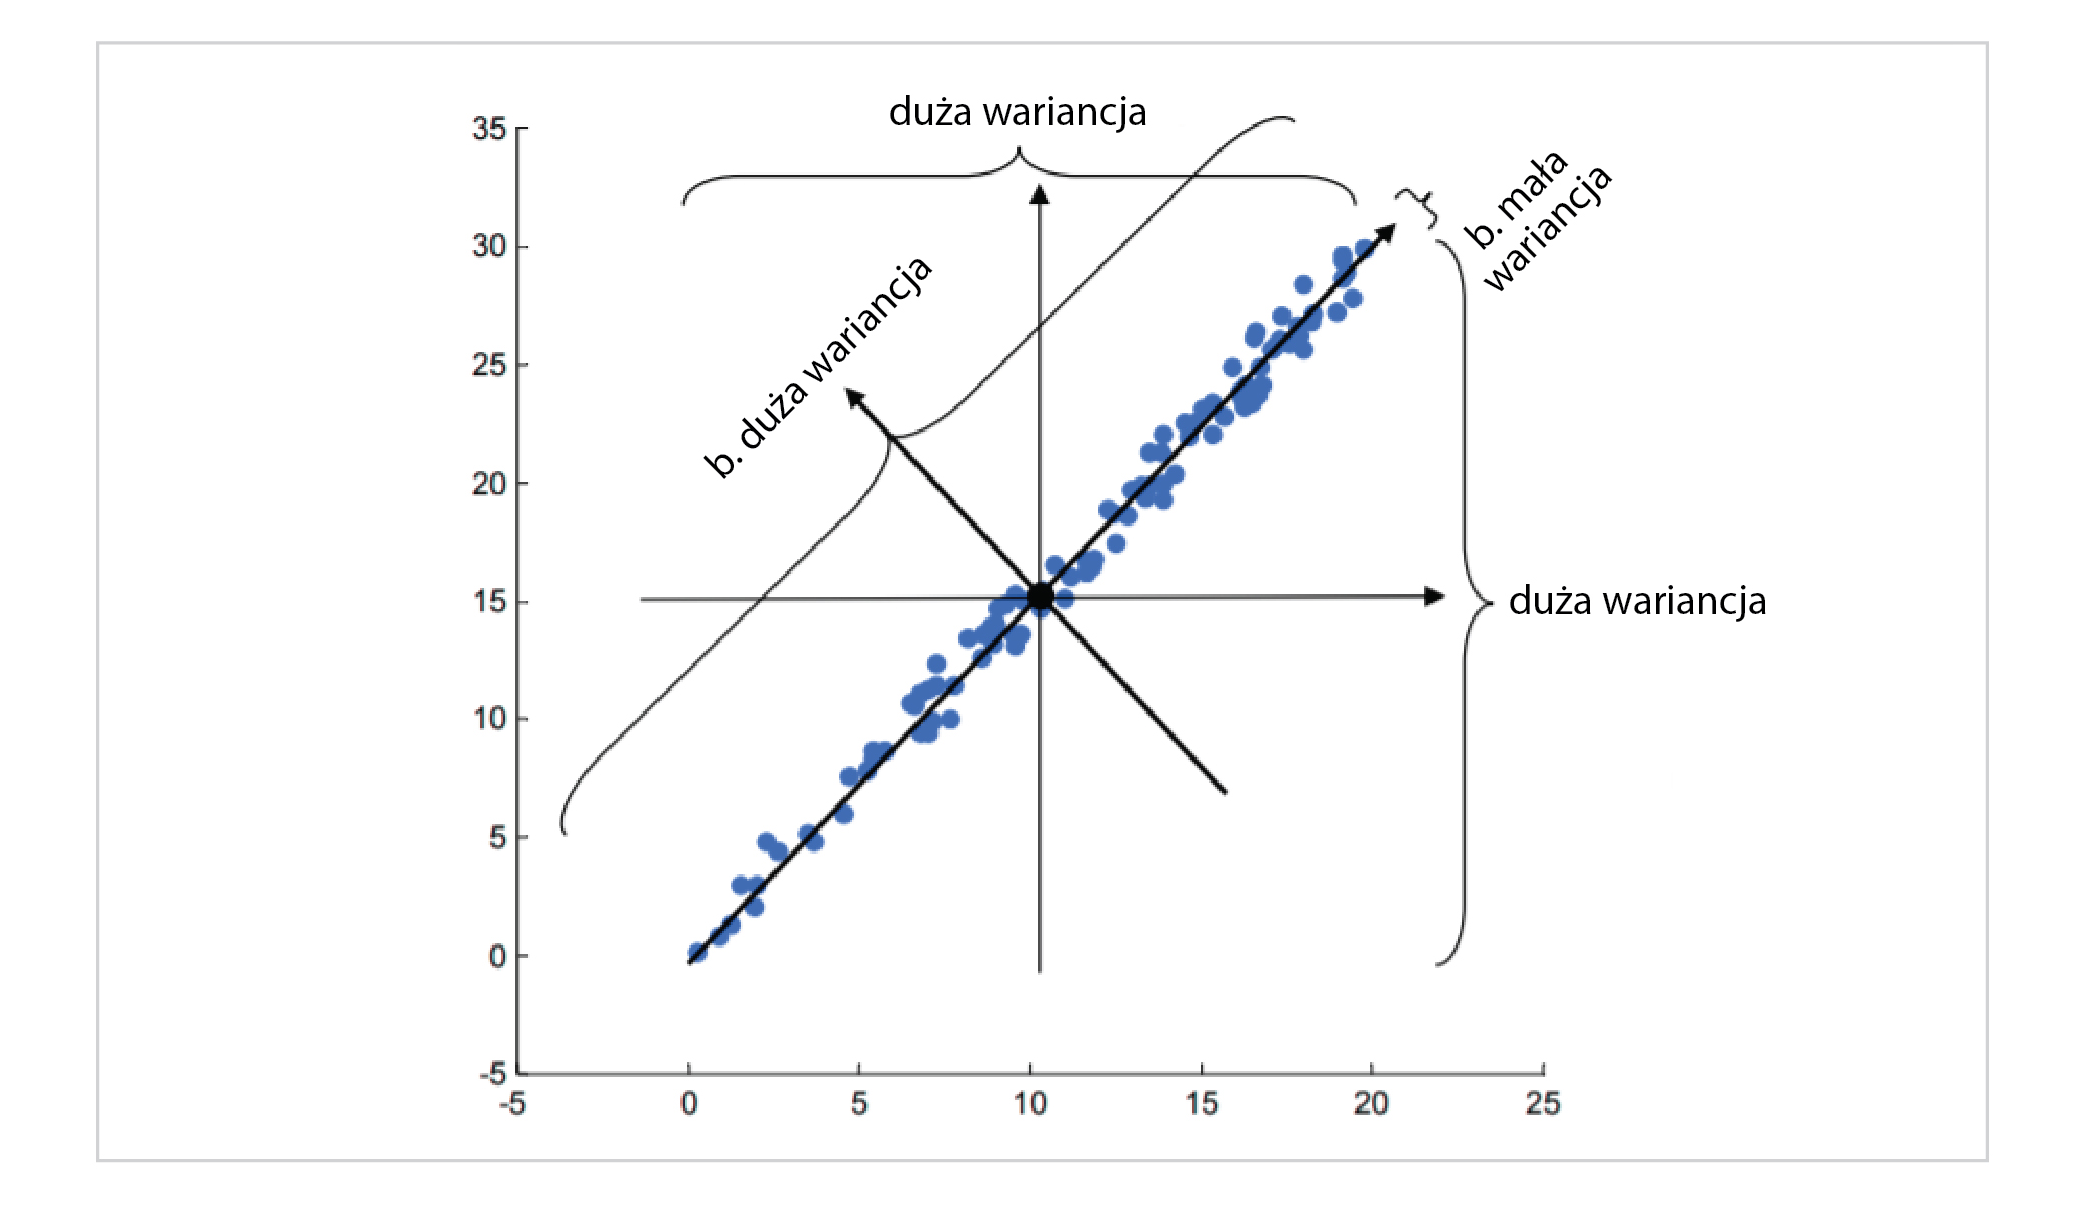
\includegraphics[width=1\textwidth]{figures/PCA.png}
	\caption{Dwuwymiarowa przestrzeń cech wraz z zaznaczonymi poziomami warianci i składowymi głównymi.}
	\label{PCA-2dim}
\end{figure}
Można zaobserwować, że nowa przestrzeń charakteryzuje się znacznie większym zróżnicowaniem poziomu wariancji niż przestrzeń oryginalna. Wybierając zatem tylko pierwszą składową uzyskana zostanie reprezentacja \textit{skomprymowana stratnie} (tzn. taka, która nie daje gwarancji odtworzenia oryginalnych wartości), ale za to zachowująca znaczną część wariancji.

Opis szczegółowej procedury PCA wygląda następująco:
\begin{enumerate}
\item Oblicz macierz kowariancji: $S_x$ = $X^{T}X$, gdzie $X$ to macierz danych zawierająca obserwacje w wierszach. Macierz $S_x$ jest symetryczna i pozwala ocenić: (1) wariancje zmiennych poprzez analizę elementów na głównej przekątnej; (2) zależności pomiędzy zmiennymi poprzez analizę elementów poza główną przekątną. 
\item Dokonaj diagonalizacji: $S_x$ = $KLK^{-1}$, gdzie $L$ to macierz diagonalna, a $K$ to macierz odwracalna składająca się z wektorów własnych odpowiadających kolejnym wartościom własnym.
\item Utwórz macierz nowych zmiennych wykonując operację: $Y$ = $XK$
\end{enumerate}

Oprócz PCA, w kontekście redukcji wymiarowości, można również wyróżnić następujące algorytmy: 
\begin{enumerate}
	\item \textit{Multidimensional scaling}, MDS -- bazuje na wyliczeniu odpowiednio zdefiniowanego dystansu między wartościami cech w oryginalnej przestrzeni i próbie zachowania tego dystansu w zredukowanej wymiarowości (zob. \cite{Chen:2008:HDV:1370965}).
	\item \textit{T-distributed stochastic neighbor embedding}, t-SNE -- stosowany do wizualizacji struktur cech w różnych skalach (zob. \cite{vanDerMaaten2008}).
	\item \textit{Isomap} -- algorytm nieliniowej redukcji wymiarowości pozwalający na gwarantowane znalezienie globalnego minimum (zob. \cite{tenenbaum_global_2000}). 
	\item \textit{Independent Component Analysis}, ICA -- stosowany do znalezienia reprezentacji danych składających się z niezależnych elementów (zob. \cite{ICA}).
	\item \textit{Latent Semantic Analysis}, LSA -- stosowany głównie w problemach dotyczących przetwarzania języka naturalnego, zwłaszcza do znalezienia kontekstu użycia danego słowa poprzez analizę statystyczną dużych bloków tekstów (zob. \cite{Wolfe2003}). 
	\item \textit{Self Organizing Maps}, SOM --  bazuje na zachowaniu własności topologicznych przestrzeni cech oryginalnych w zredukowanej wymiarowości (zob. \cite{Vesanto00self-organizingmap}).
\end{enumerate}

Zarówno przekleństwo wymiarowości, jak i wcześniej opisany problem nadmiernego dopasowania są zjawiskami bardzo często występującymi w praktycznych zastosowaniach algorytmów głębokiego uczenia się. Nie wyczerpują one jednak tematu. Szereg kolejnych wyzwań i rozwiązań został opisany w kolejnej sekcji przy okazji przedstawienia współczesnych topologii.

\section{Przykłady współczesnych topologii}

Współczesne sieci konwolucyjne służące do klasyfikacji obrazów, podobnie jak u protoplasty tj. architektury LeNet, składają się z dwóch głównych części: ekstraktora cech i klasyfikatora. W porównaniu jednak do pierwszych topologii, różnorodność warstw uległa zwiększeniu. Do najczęściej stosowanych komponentów można zaliczyć:
\begin{itemize}
	\item \textit{warstwy konwolucyjne} -- grupują filtry używane do ekstrakcji cech obrazowych różnego poziomu (np. krawędzie, skupiska, obiekty);
	\item \textit{warstwy max-pool} -- stosowane do nieliniowej redukcji wymiarowości. Z obszaru $n\times$$n$ w obrazie wyliczana jest największa wartość $I$($x$, $y$). W praktyce zazwyczaj $n$=2, podobnie jak wartość \textit{kroku} tj. odstępu pomiędzy kolejnymi próbkowaniami funkcji $I$. W uzasadnionych przypadkach stosuje się również obliczanie średniej tzw. (\textit{Avg-pool}), Normy $L2$ i innych współczynników;
	\item \textit{warstwy aktywacji} -- zawierające funkcje aktywacji neuronów. We współczesnych architekturach zamiast funkcji sigmoidalnych czy progowych stosuje się najczęściej funkcję ReLU:
	\begin{equation}
		f(x) = \max(0, x).
	\end{equation}
	Jest ona mniej wymagająca obliczeniowo niż funkcja sigmoid, a dla współczesnych topologii o dużej liczbie parametrów testy empiryczne wykazały, że równie dobrze wpływa na uzyskiwane wyniki dokładności (zob. \cite{Krizhevsky2012}); 
	\item \textit{warstwy gęste lub z ang. fully connected}, FC -- składające się z neuronów, z których każdy jest połączony z każdym neuronem kolejnej warstwy. Występują zazwyczaj w ostatniej części sieci konwolucyjnych tj. w klasyfikatorze;
	\item \textit{warstwy normalizacji}\footnote{Coraz rzadziej stosowane w praktyce z uwagi na znikomy wpływ na rezultaty.} -- normalizujące wyjście poprzedzającej warstwy do pewnego określonego przedziału, zazwyczaj (-1,1). Przykładem jest operacja \textit{Local Response Normalization} dana wzorem:
	\begin{equation}
	\label{DLnormEquation}
	b_{x,y}^{i} = a_{x,y}^{i}/\left ( k + \alpha \sum_{j=max(0,i-n/2)}^{min(N-1,i+n/2)}(a_{x,y}^{i})^2 \right )^\beta,
	\end{equation}
	gdzie $a_{x,y}^{i}$ jest aktywacją danego neuronu, a $k$, $\alpha$, $n$ i $\beta$ to stałe dobierane empirycznie na podstawie zbioru walidacyjnego (za \cite{Krizhevsky2012}). Warstwy normalizacji wykorzystywane są w celu zrównoważenia poziomu wpływu poszczególnych neuronów na wynik końcowy.
\end{itemize}

Wprowadzenie w ostatnich latach dedykowanych dla szkolenia się głębokich sieci neuronowych rozwiązań, zarówno w warstwie sprzętowej jak i oprogramowania, umożliwiło tworzenie architektur o wysokim stopniu komplikacji. W głównej mierze rozwiązania te pozwoliły na optymalizację fazy szkolenia (omówionej w poprzedniej sekcji) jak również \textit{fazy wnioskowania}, gdzie wytrenowana sieć użyta jest do przetwarzania kolejnych obserwacji. W warstwie sprzętowej wyróżnić można dedykowane akceleratory do operacji macierzowych, takie jak w \cite{DBLP:journals/corr/abs-1803-04014}, stworzone przez firmę NVIDIA, \textit{Tensor Processing Unit} (w skr. \textit{TPU}) czy opracowane przez firmę Intel procesory Nervana \cite{Intel}. 

W warstwie oprogramowania należy wspomnieć o rozwiązaniach takich jak TensorRT \cite{TensorRT}, które minimalizują czasy przetwarzania sygnału przez wytrenowaną sieć np. stosując optymalizację reprezentacji liczb zmiennoprzecinkowych lub przetwarzanych macierzy. Dynamicznie rozwijają się również frameworki do zoptymalizowanych obliczeń z udziałem głębokich sieci neuronowych np.: Caffe, Caffe2, TensorFlow, Theano, PyTorch czy MXNet. Ich porównanie osadzone w kontekście aplikacji medycznych można znaleźć w \cite{Erickson2017}.

Postęp w rozwoju współczesnych sieci konwolucyjnych doskonale odzwierciedla progres w rezultatach konkursu ImageNet Large Scale Visual Recognition Competition (w skr. ILSVRC) przedstawiony na Rys. \ref{ILSVRC}.
\begin{figure}[h!]
	\centering
	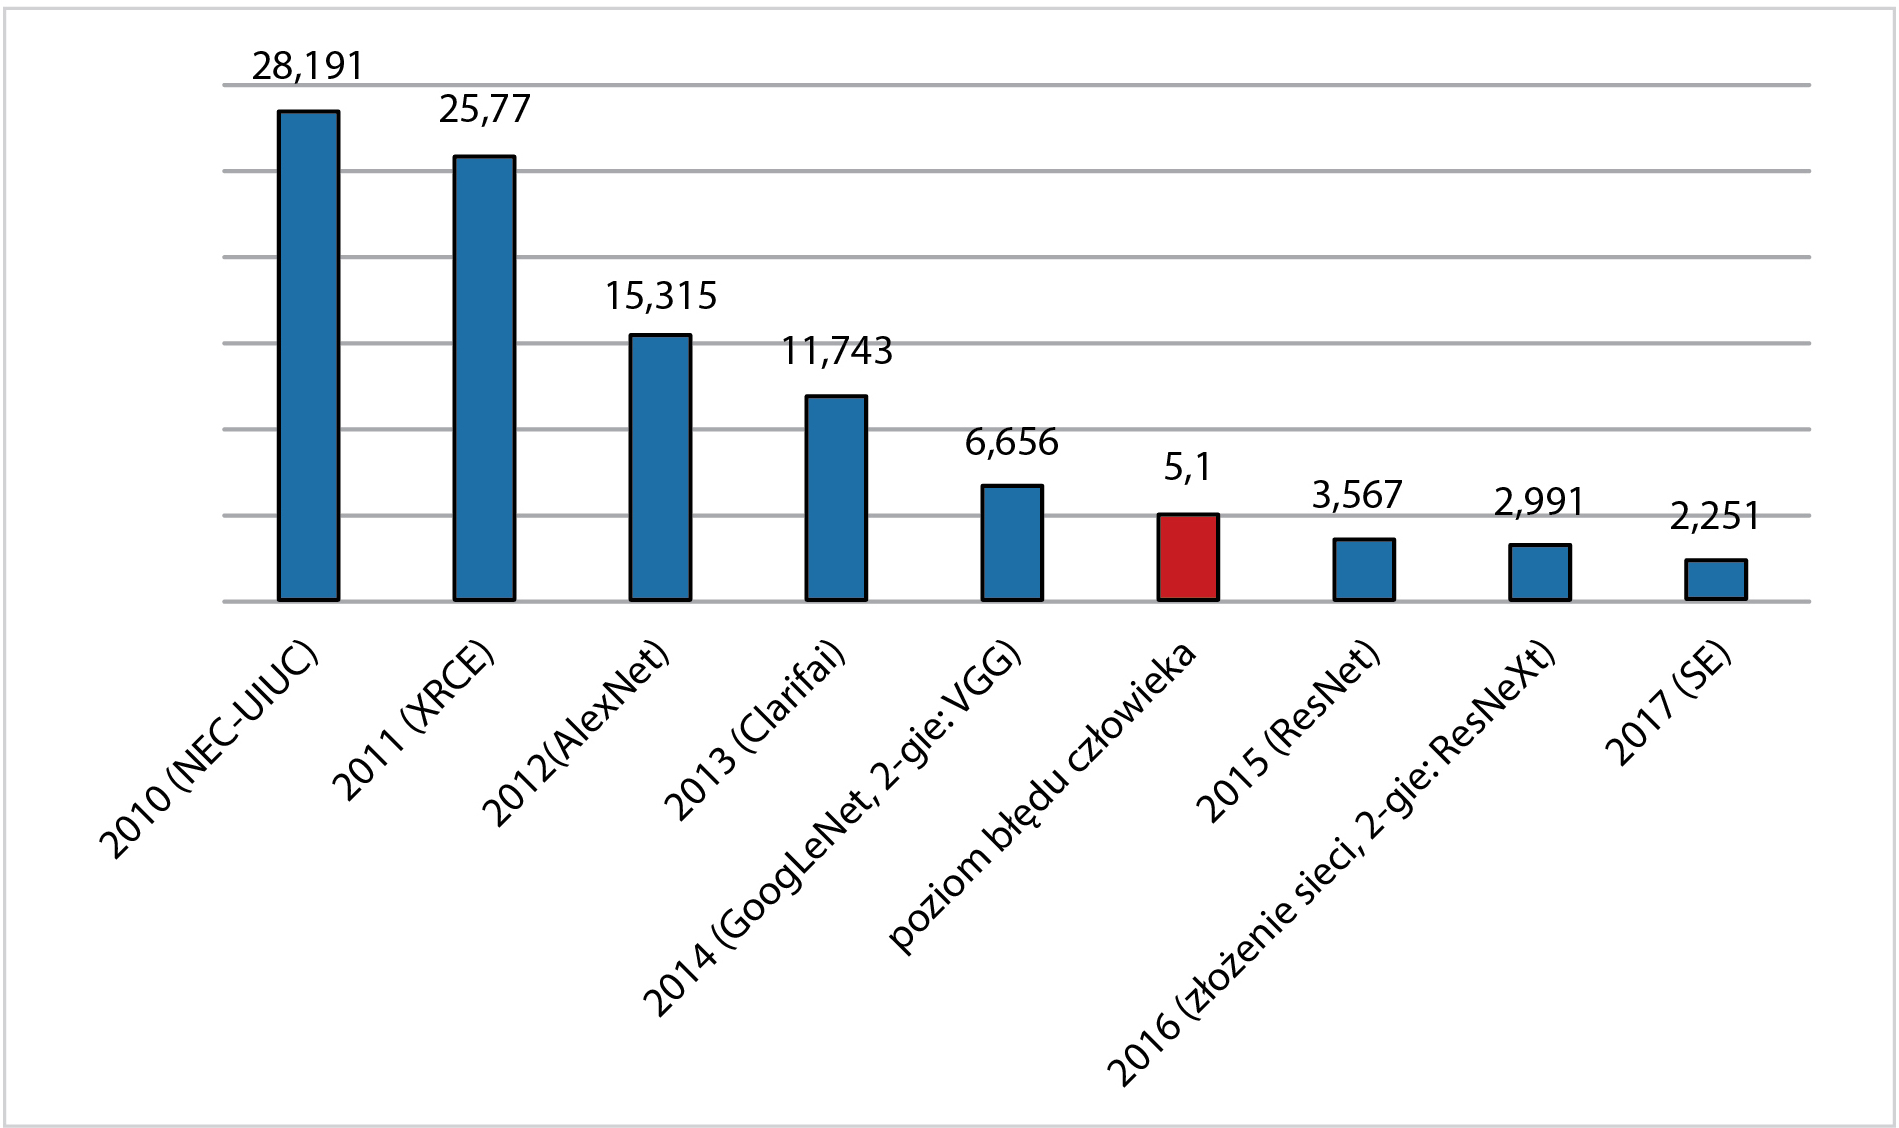
\includegraphics[width=1\textwidth]{figures/ILSVRC.jpg}
	\caption{Błąd top-5 klasyfikacji obiektów w kolejnych latach uzyskiwany przez zwycięzców konkursu ILSVRC}
	\label{ILSVRC}
\end{figure}
Prezentowane wyniki dotyczą wartości błędu klasyfikacji, na zbiorze danych \cite{imagenet_cvpr09} o nazwie ImageNet, uzyskiwanego w kolejnych latach przez zwycięskie algorytmy biorące udział w konkursie. \textit{Błąd top-$n$} należy rozumieć jako zdarzenie, w którym dla danego obrazka w $n$ wskazanych przez algorytm najbardziej prawdopodobnych etykietach nie było poprawnej. W zakresie zmniejszenia wartości błędu top-$n$, znaczący progres dokonał się w 2012 roku, gdzie błąd top-5 zmalał o 10,4 punktów procentowych, co było rezultatem działania nowej architektury sieci konwolucyjnej nazwanej AlexNet. W kolejnych latach sieci konwolucyjne deklasowały inne podejścia, doprowadzając w 2015 roku do spadku błędu top-5 do poziomu 3,5\%, co jest uznawane za poziom lepszy niż możliwości ludzkiej klasyfikacji zbioru ImageNet. Lata 2016--2018 to intensywne prace nad synergią i złożeniami różnego rodzaju modeli, które w konsekwencji doprowadziły do obniżenia wartości błędu top-5 do poziomu 2,2\%. W kolejnych podsekcjach zostanie dokładniej omówiona ewolucja zwycięskich architektur z konkursu ILSVRC. 

\subsection{AlexNet}
\label{AlexNet}
Sieć AlexNet, której nazwa pochodzi od imienia głównego twórcy tej architektury Alexa Krizhevsky, zawiera blisko 60 milionów parametrów i 650 tysięcy neuronów. Architekturę zaprezentowano na Rys. \ref{AlexNetTopology}
\begin{figure}[h!]
	\centering
	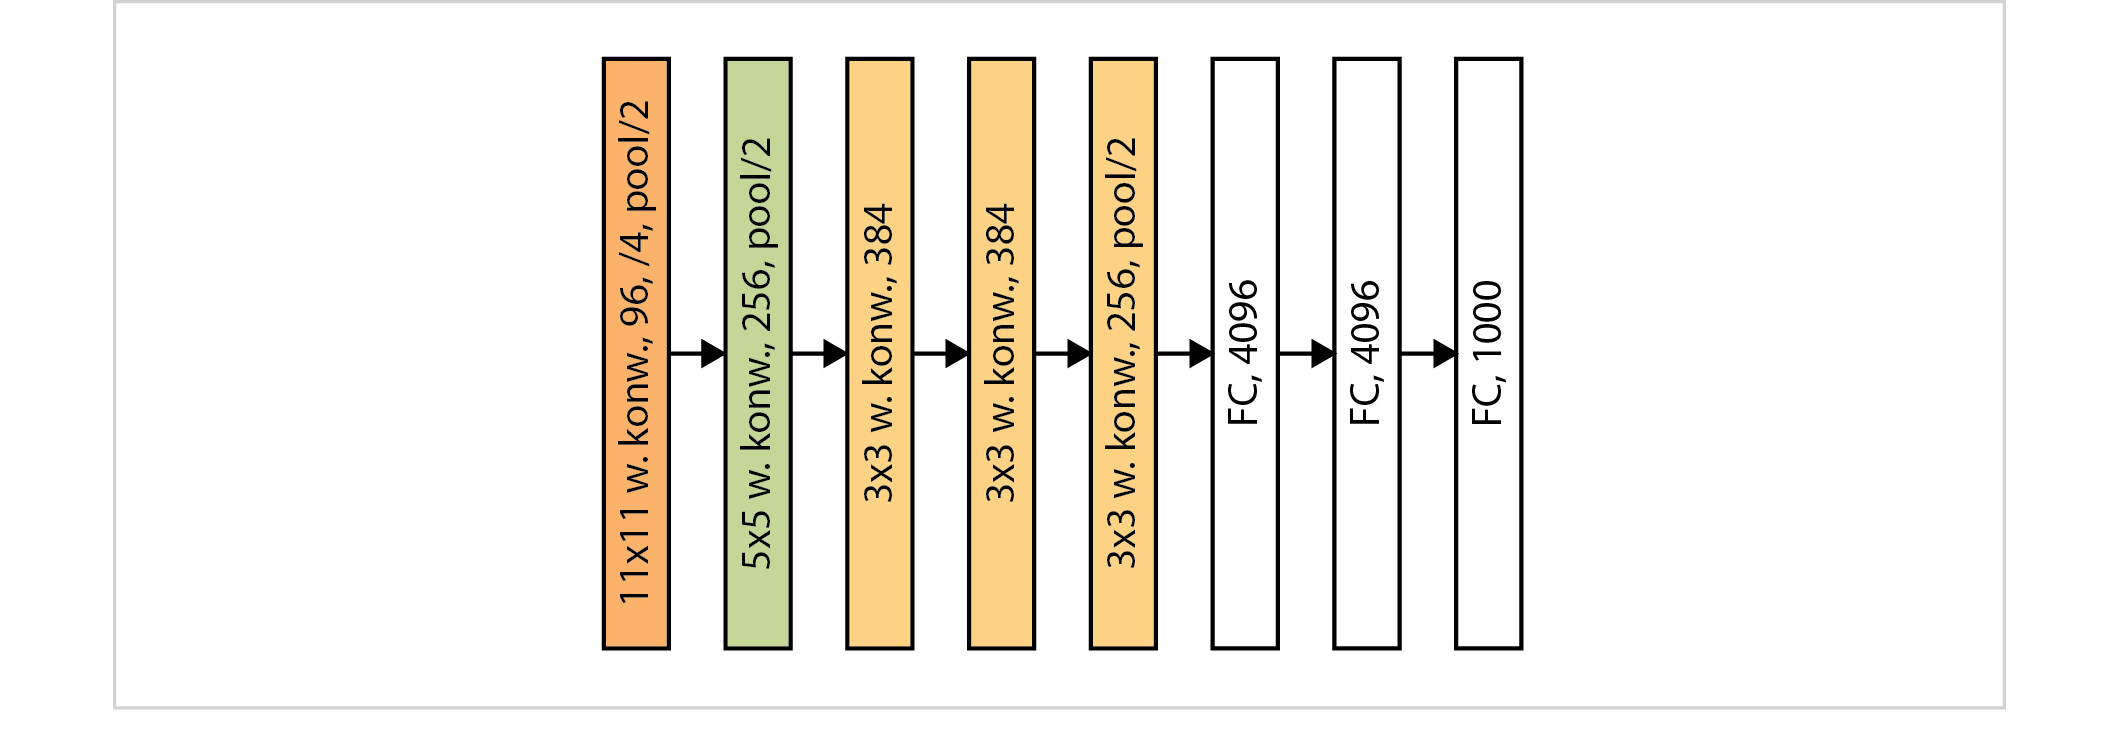
\includegraphics[width=1\textwidth]{figures/AlexNet.png}
	\caption{Schemat architektury AlexNet.}
	\label{AlexNetTopology}
\end{figure}

W skład topologii wchodzi pięć warstw konwolucyjnych i trzy gęste. Po pierwszej, drugiej i piątej warstwie konwolucyjnej występują operacje typu max-pool z maską o wymiarach 2$\times$2 \footnote{Autorzy pracy podają też przykłady użycia masek o wymiarze 2$\times$3, które nakładają się w przestrzeni funkcji obrazowej. Nie znalazły one jednak miejsca w finalnej implementacji.}. 

Pierwsza warstwa konwolucyjna przyjmuje na wejściu dane o wymiarze 227$\times$227$\times$3\footnote{3 jest liczbą kanałów kodujących kolor obrazka.}, na których wykonywana jest operacja splotu z 96 filtrami z maską o wymiarach 11$\times$11$\times$3 i krokiem 4. W rezultacie (uwzględniając również operację max-pool) objętość wynikowa przekazywana do kolejnej warstwy ma wymiar 27$\times$27$\times$96. W drugiej warstwie konwolucyjnej wykonywana jest operacja splotu z 256 filtrami z maską o wymiarach 5$\times$5$\times$96. Wymiar objętości wynikowej zostaje ponownie zredukowany poprzez operacje max-pool do 13$\times$13$\times$256. Kolejne 3 warstwy konwolucyjne są połączone bezpośrednio ze sobą. Trzecia warstwa zawiera 384 filtry z maską o wymiarze 3$\times$3$\times$256, w skład czwartej wchodzą 384 filtry z maską o wymiarze 3$\times$3$\times$384, a w piątej znajduje się 256 filtrów również z maską o wymiarze 3$\times$3$\times$384. Końcowe dwie warstwy typu FC zawierają po 4096 neuronów, a ostatnia zawiera tyle neuronów ile klas występuje w ostatecznym podziale -- w oryginalnej pracy było to 1000 (por. \cite{Krizhevsky2012}).

Poniżej przedstawiono przykład algorytmu wykorzystywanego dla pierwszej warstwy konwolucyjnej opisywanej topologii, umożliwiający zrozumienie sposobu przetwarzania sygnału wejściowego: 
\begin{enumerate}
\item Z danych wejściowych o wymiarze [227$\times$227$\times$3] wybierany jest co czwarty blok  o wymiarach [11$\times$11$\times$3] (zarówno wzdłuż wysokości jak i szerokości). W rezultacie, nie uwzględniając krawędzi obrazu, otrzymywanych jest 217 punktów w każdym rzędzie i w kolumnie, w których mieści się [55$\times$55] tj. 3025 bloków.
\item Zarówno 11$\times$11$\times$3 = 363 wagi znajdujące się w 96 filtrach jak i wartości 363 punktów obrazowych znajdujących się 3025 blokach są przedstawiane w postaci macierzy $A$ o wymiarach [96$\times$363] i $B$ o wymiarach [363$\times$3025].
\item Liczony jest iloczyn skalarny w postaci A$^\intercal$B = $C$, gdzie nowa, wyjściowa macierz $C$ ma wymiar [96$\times$3025].
\item Rezultat w postaci macierzy $C$ ponownie przewymiarowany jest na postać [55$\times$55$\times$96].  
\end{enumerate} 

W architekturze jako funkcję aktywacji neuronów wykorzystano ReLU, co znacząco przyspieszyło trening sieci. Uzyskano 6-krotne przyspieszenie treningu dla danych CIFAR-10 (zob. \cite{CIFAR}) w stosunku do tej samej topologii wykorzystującej sigmoidalną funkcję aktywacji. Ponieważ funkcja ReLU nie posiada górnego ograniczenia, neurony teoretycznie mogą posiadać nieograniczone wartości funkcji aktywacji. W celu polepszenia kontrastu pomiędzy neuronami i wydobycia tych, które na tle innych się wyróżniają, zastosowano normalizację zgodną ze wzorem \ref{DLnormEquation}. W wyniku uzyskano redukcję błędu klasyfikacji top-5 o wartość 1,2 punktu procentowego.

W kontekście zwiększenia efektywności treningu zastosowano również powiększenie rozmiaru danych poprzez rotacje i modyfikacje funkcji obrazowej z wykorzystaniem czynników głównych (zob. \cite{Krizhevsky2012}) zmniejszając błąd top-1 o 1\%. Zastosowano też technikę dropout opisaną w \ref{sec-overffiting}. Ostatecznie wprowadzono także trening z wykorzystaniem wielu GPU (zob. Rys. \ref{AlexNetTopologyMultiGPU}). 

\begin{figure}[h!]
	\centering
	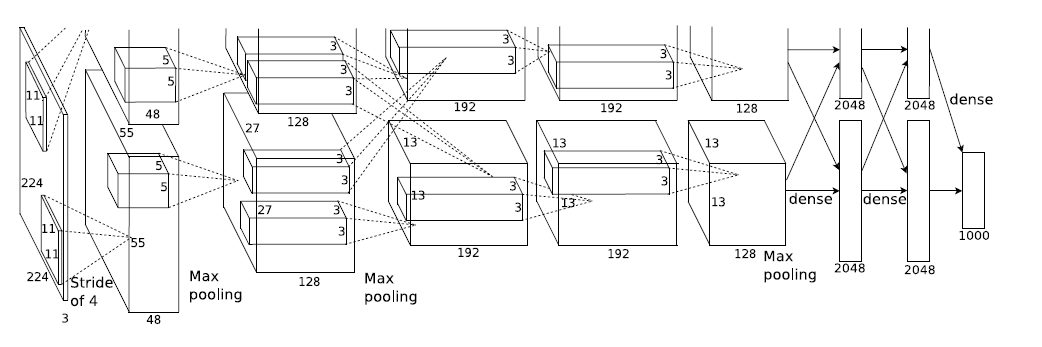
\includegraphics[width=1\textwidth]{figures/AlexNet-multiGPU.png}
	\caption{Topologia architektury AlexNet z podziałem na dwa akceleratory GPU.}
	\label{AlexNetTopologyMultiGPU}
\end{figure}

Topologia z podziałem na 2 karty zwiększyła dwukrotnie sumaryczną pamięć i pozwoliła na kolokację parametrów sieci.

Praca Alexa Krizhevsky, Ilya Sutskever i Geoffrey'a Hinton zapoczątkowała wzrost zainteresowania technikami głębokiego uczenia się, co doprowadziło do publikacji kolejnych podobnych architektur. Do najbardziej znanych należą ZFNet z 2013 roku \cite{ZFNet}, gdzie m.in. zastosowano zmniejszenie wymiaru maski stosowanego w filtrach pierwszej warstwy konwolucyjnej do 7$\times$7 oraz VGGNet \cite{VGGNet} z 2014 roku, gdzie zastosowano większą liczbę warstw konwolucyjnych z mniejszym wymiarem maski. Również w 2014 roku zaprezentowano innowacyjną koncepcję modułów sieci konwolucyjnych, co doprowadziło do zwycięstwa w ILSVRC. Idea ta została dokładniej opisana w kolejnej podsekcji.

\subsection{GoogLeNet}
\label{googlenet}
Architekturę o nazwie GoogLeNet zaprezentowano w 2014 r. w pracy \cite{GoogleNet}. Nazwa architektury pochodzi od nazwy zwycięskiego zespołu startującego w ILSVRC 2014, składającego się z pracowników firmy Google. Oryginalnie topologia składała się z 22 warstw i zawierała około 5 mln parametrów (12 razy mniej niż w przypadku sieci AlexNet). 

Redukcję liczby parametrów przy jednoczesnym podwyższeniu dokładności klasyfikacji obiektów udało się uzyskać poprzez poszukiwania konstrukcji optymalnych lokalnych topologii i ich połączeń. Mianowicie, wiadomo że duża część funkcji aktywacji neuronów przyjmuje wartość 0 lub jest redundantna z powodu wysokiej korelacji między sobą (zob. \cite{DBLP:journals/corr/AroraBGM13}). Matematyka dotycząca przetwarzania \textit{macierzy rzadkich}, tj. gdzie przeważająca liczba elementów przyjmuje wartość 0, jest dobrze znana (zob. np. \cite{Umit2010}). Jednak implementacje bibliotek do obliczeń związanych z algebrą liniową są zoptymalizowane pod kątem \textit{macierzy gęstych}, gdzie przeważająca liczba elementów przyjmuje wartości różne od 0 (zob. \cite{Song:2014:SUM:2597652.2597670, Krizhevsky2012}). 

Ideą modułu incepcji zaproponowanego przez twórców GoogLeNet jest aproksymacja rzadkich macierzy z użyciem komponentów o gęstej strukturze. Takie komponenty nazwano \textit{modułami incepcji} (ang. \textit{inception modules}), a ich przykłady pokazano na Rys. \ref{GoogleNetInceptionModules}. 
\begin{figure}[h!]
	\centering
	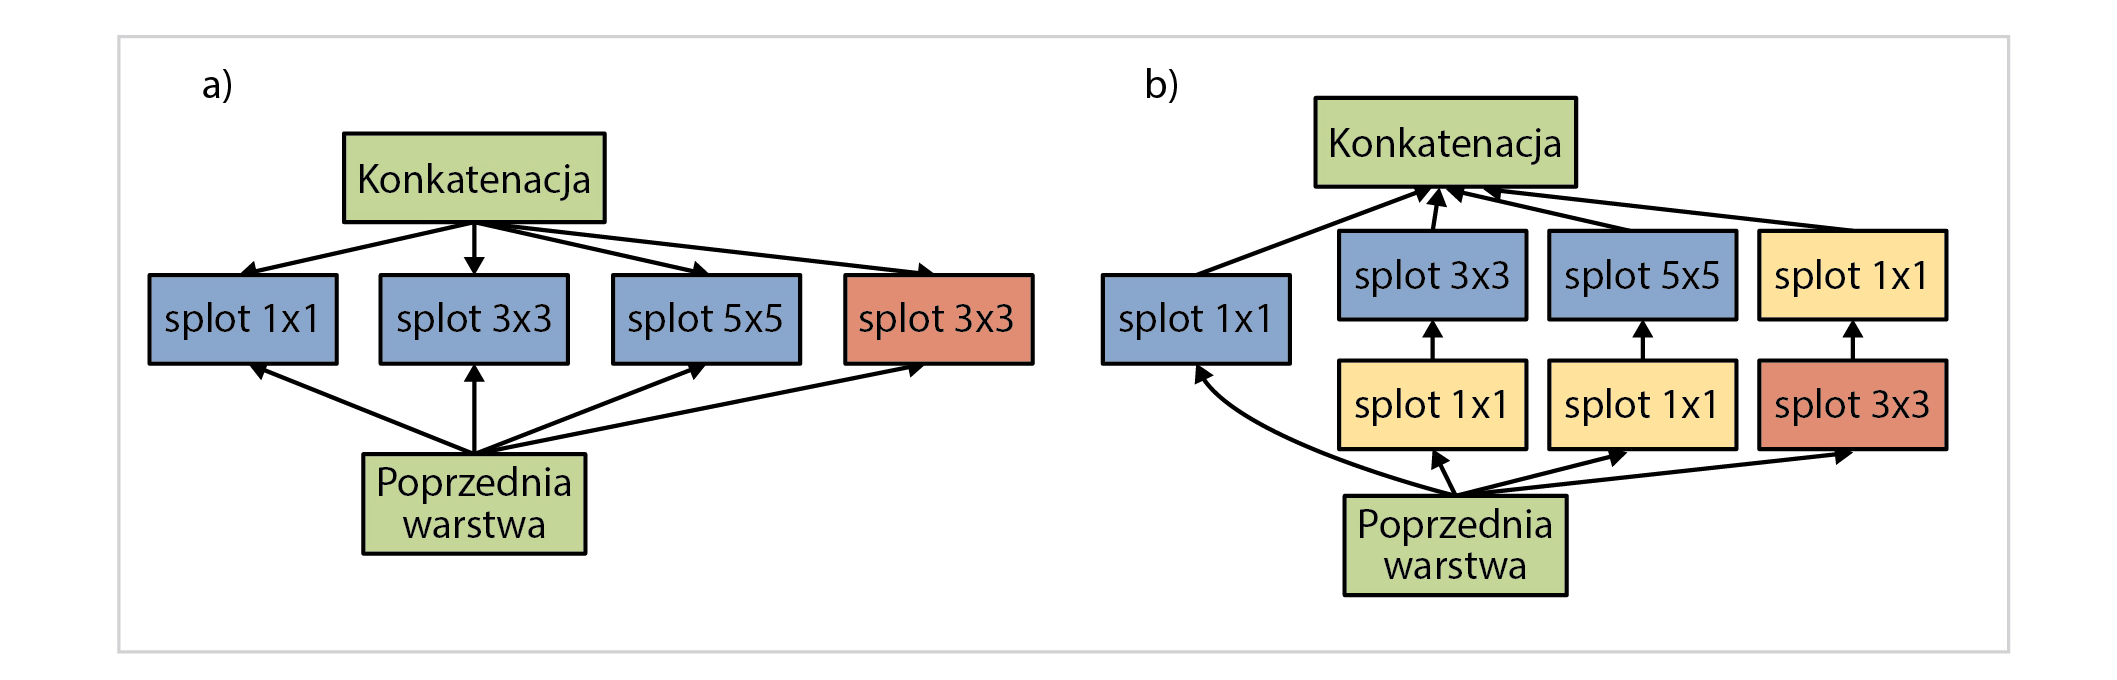
\includegraphics[width=1\textwidth]{figures/InceptionModules.png}
	\caption{Moduły incepcji o głębokości jednego (po lewej) i dwóch stopni (po prawej).}
	\label{GoogleNetInceptionModules}
\end{figure}

(a) przedstawia naiwną formę modułu incepcji, gdzie grupowane są operacje filtrów z maską o wymiarach 5$\times$5, 3$\times$3, 1$\times$1 oraz operacja max-pool. (b) prezentuje koncepcję zoptymalizowaną obliczeniowo gdzie filtry z maską 1$\times$1 służą do redukcji wymiarowości i używane są bezpośrednio przed splotami z bardziej wymagającymi obliczeniowo splotami 5$\times$5 i 3$\times$3. 

Przy pomocy złożenia różnego rodzaju modułów incepcji otrzymano topologię zaprezentowaną na Rys. \ref{GoogleNetTopo}.
\begin{figure}[h!]
	\centering
	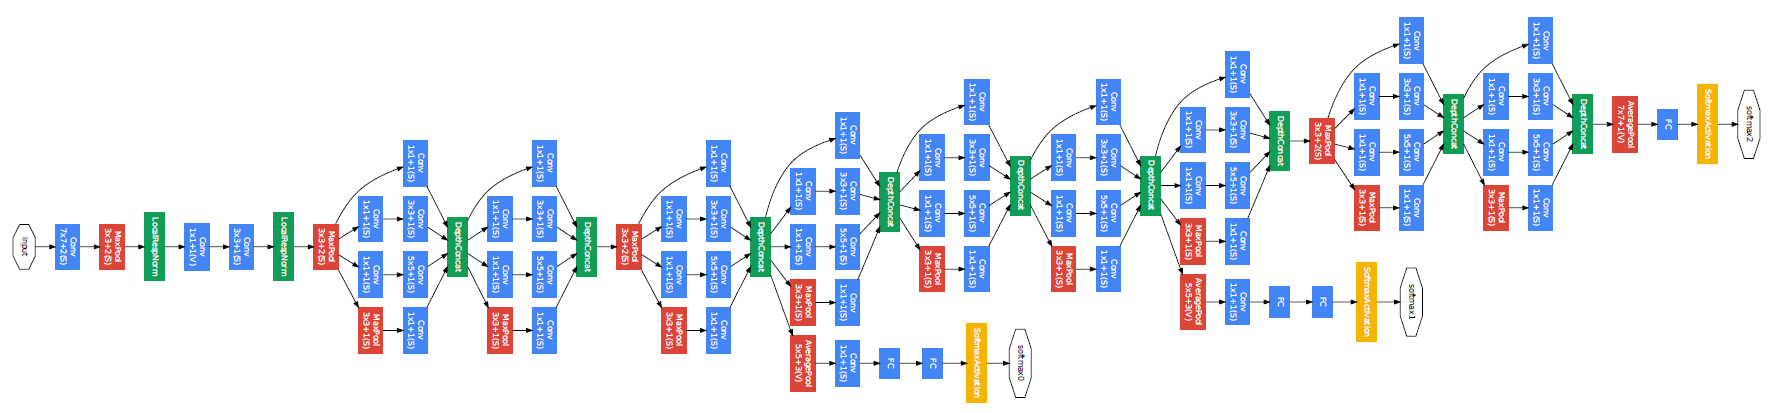
\includegraphics[width=1\textwidth]{figures/GoogleNet.png}
	\caption{Topologia architektury GoogleNet}
	\label{GoogleNetTopo}
\end{figure}
Zestawienie jej parametrów znajduje się w Tabeli \ref{GoogleNetParams}.
\renewcommand{\arraystretch}{1.2}
\begin{table}[h!]
	\setlength{\tabcolsep}{14pt}
	\centering
	\caption{Parametry architektury GoogleNet}
	\scriptsize
	\label{tab:USG-params}
	\begin{tabular}{l | c | c | c | c }
		%\hline
		Typ warstwy  & Wymiar  & Wymiar & Głębokość & Liczba   \\  
		& maski/krok & wyjściowy &&parametrów\\
	    \hline \hline
		Konwolucyjna   & 7$\times$7/2 & 112$\times$112$\times$64 & 1 & 2,7K \\ \hline
		Max-pool & 3$\times$3/2 & 56$\times$56$\times$64 & 0 & --  \\ \hline
		Konwolucyjna & 3$\times$3/2 & 56$\times$56$\times$192 & 2 & 112K  \\ \hline
		Max-pool & 3$\times$3/2 & 28$\times$28$\times$192 & 0 & --  \\ \hline
		M. incepcji & -- & 28$\times$28$\times$256 & 2 & 159K  \\ \hline
		M. incepcji & -- & 28$\times$28$\times$480 & 2 & 380K  \\ \hline
		Max-pool & 3$\times$3/2 & 14$\times$14$\times$480 & 0 & --  \\ \hline
		M. incepcji & -- & 14$\times$14$\times$512 & 2 & 364K  \\ \hline
		M. incepcji & -- & 14$\times$14$\times$512 & 2 & 437K  \\ \hline
		M. incepcji & -- & 14$\times$14$\times$512 & 2 & 463K  \\ \hline
		M. incepcji & -- & 14$\times$14$\times$528 & 2 & 580K  \\ \hline
		M. incepcji & -- & 14$\times$14$\times$832 & 2 & 840K  \\ \hline
		Max-pool & 3$\times$3/2 & 7$\times$7$\times$832 & 0 & --  \\ \hline
		M. incepcji & -- & 7$\times$7$\times$832 & 2 & 1072K  \\ \hline
		M. incepcji & -- & 7$\times$7$\times$1024 & 2 & 1388K  \\ \hline
		Avg-pool & 7$\times$7/2 & 1$\times$1$\times$1024 & 0 & --  \\ \hline
		Dropout (40\%) & -- & 1$\times$1$\times$1024 & 0 & --  \\ \hline
		Warstwa aktywacji & -- & 1$\times$1$\times$1000 & 1 & 1000K  \\ \hline
	\end{tabular}
	\label{GoogleNetParams}
\end{table}
\renewcommand{\arraystretch}{1}
Ważną cechą sieci GoogleNet jest brak warstw typu FC na zakończeniu, gdzie w przypadku sieci AlexNet znajduje się około 90\% parametrów. Końcowe wnioskowanie jest realizowane na podstawie wartości średniej z dwuwymiarowych map cech.

Dla lepszego zrozumienia idei redukcji wymiarowości realizowanej przez moduły incepcji, podobnie jak w przypadku sieci AlexNet, przeanalizowane zostanie działanie pierwszego modułu w topologii z Rys. \ref{GoogleNetTopo}.
Moduł zawiera 128 filtrów z maskami o wymiarach 3$\times$3 i 32 filtry z maskami o wymiarach 5$\times$5. Dane na wejściu modułu mają 192 kanały (zob. Tabela \ref{GoogleNetParams}). Dla przykładu, rząd wielkości obliczeń operacji splotów 32 filtrów 5$\times$5 wynosi 25$\times$32$\times$192=153 600 i dalej wzrastałby z głębokością sieci. W celu zapobiegnięcia nadmiarowi obliczeń stosowana jest redukcja z użyciem 16 filtrów z maską o wymiarach 1$\times$1. W efekcie rząd wielkości obliczeń spada do 16$\times$192 +  25$\times$32$\times$16=15 876, co pozwala na dalsze budowanie wielowarstwowych struktur.

Topologia GoogLeNet jest wciąż rozwijana. Po pierwszej prezentacji pojawiły się kolejne modernizacje wprowadzające dodatkowe faktoryzacje modułów jak w Inception-v2 lub normalizacje wartości wynikowych poszczególnych warstw jak w Inception-v3. Obie sieci zostały przedstawione w \cite{DBLP:journals/corr/SzegedyVISW15}. Kolejny innowacyjny pomysł, bazujący na dodatkowych połączeniach między blokami, został wprowadzony w 2015 roku w sieci ResNet opisanej w kolejnej podsekcji.

\subsection{ResNet}
\label{resnet}
Jednym z najbardziej oczywistych pomysłów na polepszenie dokładności działania sieci neuronowych jest zwiększenie liczby warstw. Jednak wraz ze wzrostem liczby warstw, trening takich architektur z użyciem tradycyjnych metod gradientowych (takich jak algorytm wstecznej propagacji błędu) staje się mniej wydajny. Problem wynika z faktu, że zmiana wartości sygnału na wyjściu sieci w odpowiedzi na sygnał wejściowy jest mniejsza wraz ze wzrostem liczby warstw. W takiej sytuacji gradient wyliczany na podstawie sygnału będącego różnicą pomiędzy sygnałem wejściowym a wyjściowym może przyjmować wartości bliskie 0 uniemożliwiając dalszy postęp uczenia się. Problem zanikającego gradientu (ang. \textit{vanishing gradient problem}) rozwiązywany jest poprzez zastosowanie normalizacji oraz nieliniowych funkcji aktywacji. Dzięki tym mechanizmom algorytm treningu głębokich sieci neuronowych w większej liczbie przypadków zbiega do użytecznego minimum lokalnego. 

W momencie znalezienia takiego minimum dodanie kolejnych warstw i parametrów sieci jest redundantne, a nawet prowadzi do pogorszenia wyników treningu sieci. Zjawisko to nosi nazwę \textit{degradacji treningu} (ang. \textit{degradation problem}). Twórcy architektury ResNet, przedstawionej w \cite{ResNet}, zaproponowali rozwiązanie tego problemu poprzez implementację bloków rezydualnych (ang. \textit{Residuum Units}) zawierających dodatkowe, skrótowe połączenia (ang. \textit{skip conections}) pomiędzy wejściem a wyjściem bloków. Porównanie schematów funkcjonalnych nowych bloków i wcześniej istniejącego rozwiązania stosowanego np. w AlexNet zostało przedstawione na Rys. \ref{ResNetBlock}.
\begin{figure}[h!]
	\centering
	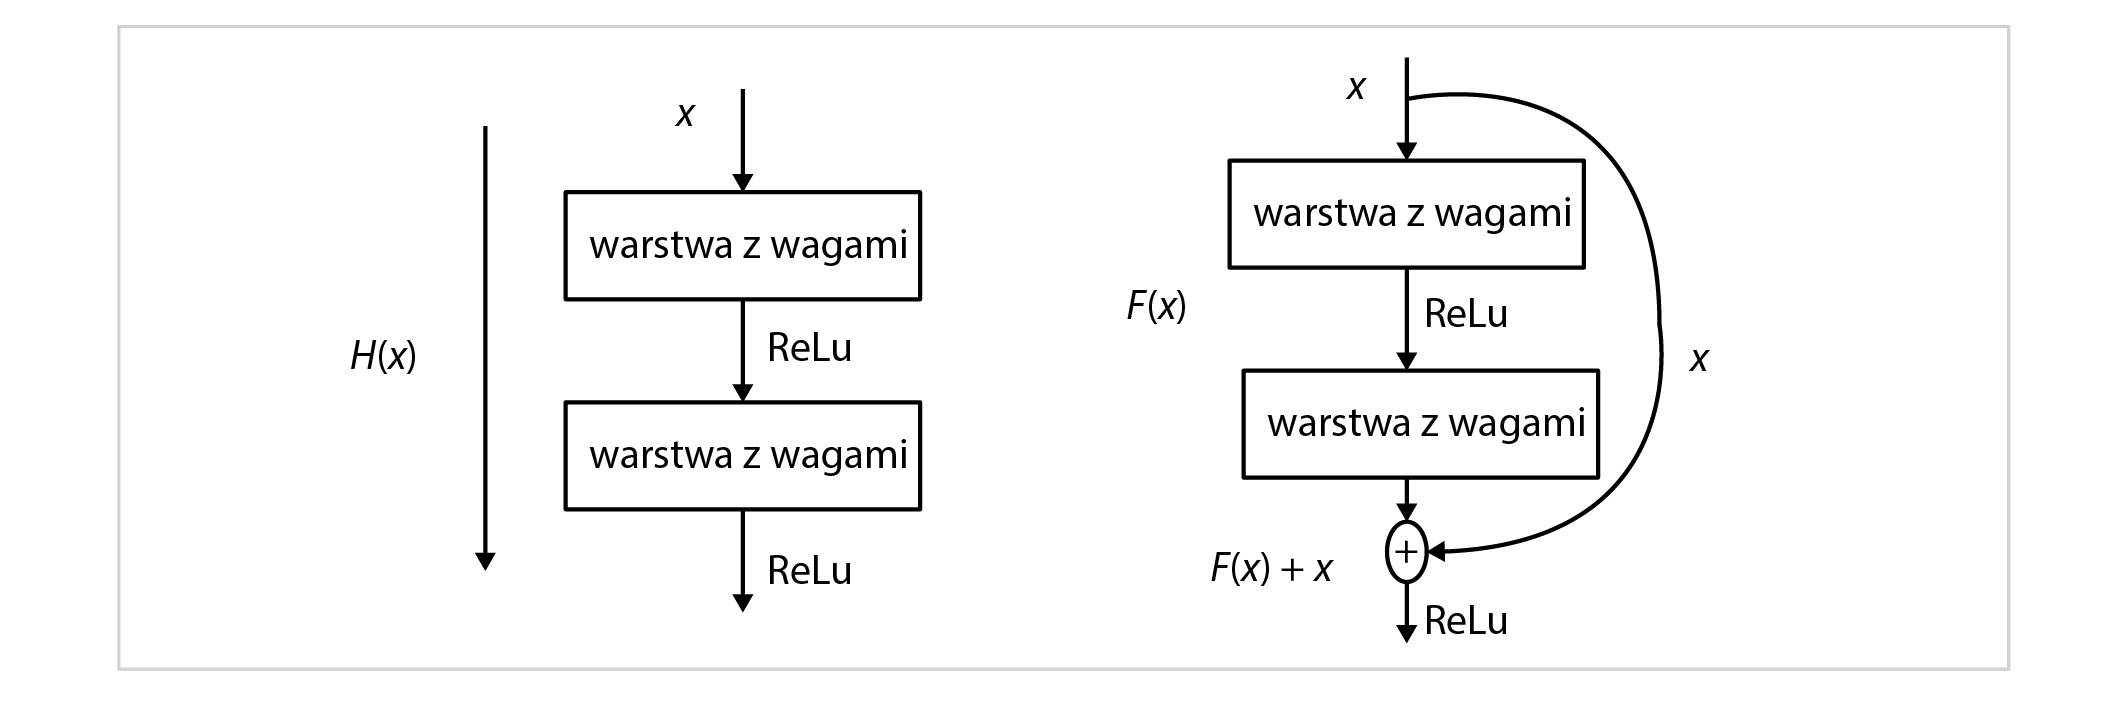
\includegraphics[width=1\textwidth]{figures/ResidualBlock.png}
	\caption{Schemat funkcjonalny pojedynczego bloku w architekturze ResNet.}
	\label{ResNetBlock}
\end{figure} 

Ogólną postać równania bloku rezydualnego można zapisać następująco:
\begin{equation}
\begin{split}
y_l = h(x_l) + F(x_l, W_l),\\
x_{l+1} = f(y_l),
\end{split}
\end{equation}
gdzie $x_l$ i $x_{l+1}$ stanowią sygnał wejściowy i wyjściowy $l$-tego bloku. $F$ stanowi funkcję rezydualną optymalizowaną podczas treningu sieci, $h$($x_l$) stanowi funkcję przekształcenia sygnału $x_l$ przekazywanego skrótowym połączeniem, $f$ jest funkcją ReLU, a $W$ stanowi macierz wag.

Funkcja $h$($x_l$) jest funkcją tożsamościową, a zatem $h$($x_l$) = $x_l$. Żeby uzasadnić ten wybór należy rozważyć propagację gradientu wewnątrz sieci składającej się z bloków rezydualnych. Dla każdego $L$-tego bloku zachodzi równanie:
\begin{equation}
x_L = x_l + \sum_{i=l}^{L-1}F(x_i, W_i)
\end{equation}
Korzystając z reguły łańcuchowej można zapisać równanie na gradient funkcji kosztu $\varepsilon$:
\begin{equation}
\label{gradResBlock}
\frac{\partial \varepsilon}{\partial x} =  \frac{\partial \varepsilon}{\partial x_L} \frac{\partial x_L}{\partial x_l} =  \frac{\partial \varepsilon}{\partial x_L}\left (1 +   \frac{\partial }{\partial x_l}\sum_{i=l}^{L-1}F(x_i, W_i) \right )
\end{equation}
z czego wynika, że gradient może być podzielony na dwie addytywne składowe: (1) $w$ = $\frac{\partial \varepsilon}{\partial x_L}$ propagowaną bez wpływu na warstwy zawierające wagi i (2) $\lambda$ = $\frac{\partial \varepsilon}{\partial x_L}\frac{\partial }{\partial x_l}\sum_{i=l}^{L-1}F(x_i, W_i)$ propagowaną przez nie.

Przykład propagacji gradientu w sieci składającej się z trzech bloków wygląda zatem następująco:
\begin{equation}
\label{gradRes3Block}
\frac{\partial \varepsilon}{\partial x_0} =  \frac{\partial \varepsilon}{\partial x_3}*(w_2+\lambda_2)*(w_1+\lambda_1)*(w_0+\lambda_0)
\end{equation}

Wartości $w$ są zazwyczaj znormalizowane do przedziału (-1;1) można więc rozważyć 4 istotne przypadki równania \ref{gradRes3Block}:
\begin{enumerate}
	\item $\lambda$ = 0 -- nie ma skrótowych połączeń, co odpowiada płaskiej strukturze sieci. Ponieważ wartości $w$ są z przedziału (-1;1) dodawanie kolejnych warstw wzmacnia wcześniej omówiony efekt zanikającego gradientu
	\item $\lambda$ $>$ 1 -- z każdą warstwą, sumaryczna wartość gradientu zwiększa się inkrementalni, co nazywane jest \textit{problemem eksplozji gradientu} (ang. \textit{exploding gradient problem}).
	\item $\lambda$ $<$ 1 -- przy założeniu, że $w$ + $\lambda$ $<$ 1, dla sieci składających się z wielu warstw występuje problem zaniku gradientu, jak w przypadku 1. Natomiast, gdy $w$ + $\lambda$ $>$ 1 podobnie jak w przypadku 2 może występować problem eksplozji gradientu
	\item $\lambda$ $=$ 1 -- wartości $w$ są inkrementowane dokładnie o 1, co eliminuje problemy podane w przypadkach 1, 2 i 3 i stanowi uzasadnienie dla wyboru funkcji tożsamościowej $h$($x_l$) w architekturze ResNet.
\end{enumerate}

Dokładny opis matematyczny funkcjonowania bloków rezydualnych wraz z dowodami znajduje się w \cite{DBLP:journals/corr/HeZR016}. Przykład topologii sieci składającej się z 8 bloków i łącznie 18 warstw tzw. ResNet-18, przedstawiono na Rys. \ref{ResNetTopo}.
\begin{figure}[h!]
	\centering
	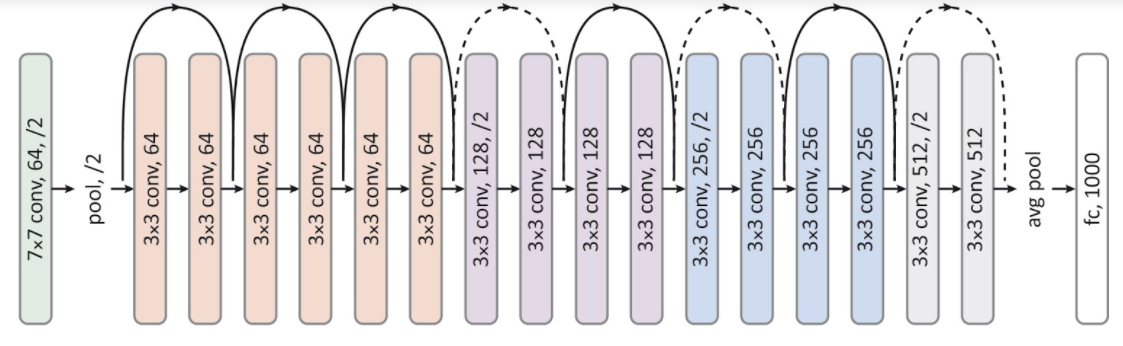
\includegraphics[width=1\textwidth]{figures/ResNet.png}
	\caption{Topologia architektury ResNet-18.}
	\label{ResNetTopo}
\end{figure} 

Pierwsza warstwa konwolucyjna zawiera filtry z maską o wymiarach 7$\times$7. W kolejnych zastosowano wymiar 3$\times$3. Zastosowanie mniejszych wymiarów masek niż w AlexNet oraz podobnie jak w przypadku sieci GoogLeNet wyliczenie na końcu wartości średniej z dwuwymiarowych map cech zredukowało liczbę parametrów.

Architektura ResNet-18 jest najmniejszą z pojawiających się w literaturze przykładów tego typu. W praktyce, z powodzeniem wykorzystywano topologie składające się nawet z 1202 warstw (zob. \cite{ResNet}). W 2016 roku zaprezentowano w \cite{InceptionResNet} hybrydę sieci GoogleNet i ResNet. Pracowano również nad bardziej złożonymi blokami, co w konsekwencji doprowadziło w 2017 roku do zaprezentowania architektury ResNetX w \cite{ResNetX}, która w wielu testach klasyfikacji różnych zbiorów okazała się być lepsza niż poprzednicy. Przegląd dotyczący historii tych prac można znaleźć w \cite{ResNetXoverview}.

Sieć ResNet i jej warianty dla wielu testowych zbiorów danych takich jak ImageNet, CIFAR czy COCO \cite{COCO} osiągnęły dokładność klasyfikacji porównywalną z możliwościami ludzkiego obserwatora. Dalszy progres był możliwy m.in. dzięki zastosowaniu synergii wielu modeli, co zostało opisane w kolejnej podsekcji.

\subsection{Złożenia}
Uczenie złożeń sieci (ang. \textit{esemble learning}) polega na wykorzystywaniu kilku modeli bazowych i wybranej metody ich synergii. W kontekście głębokiego uczenia się stosowane są różne metody kombinacji modeli bazowych (zob. \cite{Ensemble}). Jako często stosowane przykłady można podać: uśrednianie, głosowanie, klasyfikacja Bayesa, generalizację stosów. Zostaną one kolejno omówione:

\subsubsection{Uśrednianie}
Uśrednianie jest prostą metodą kombinacji wyników predykcji. Najczęściej stosowane jest uśrednienie bez wag, gdzie suma wyników predykcji modeli bazowych podzielona jest przez ich liczbę. Uśredniać można bezpośrednio wyniki ostatecznej klasyfikacji jak również prawdopodobieństwa przynależności do odpowiednich klas, które są np. wynikiem \textit{funkcji softmax}:
\begin{equation}
\sigma (z)_j= \frac{e^{z_j}}{\sum_{k=1}^{K} e^{z_k}},
\end{equation} 
używanej często bezpośrednio przed ostatnią warstwą sieci neuronowych dla $z$ sygnałów wejściowych i $j$ wyjściowych.

Główną zaletą uśredniania jest redukcja wariancji. Jest ona tym większa im bardziej nieskorelowane są wyniki predykcji modeli bazowych. Pomimo prostoty, tego rodzaju koncepcja odnosiła już sukcesy m.in. w lasach losowych (zob. \cite{Breiman2001}).

Zastosowanie uśredniania przy silnie odstających od średniej najgorszych predykcjach znacząco obniża dokładność całego złożenia. Dlatego przy tak nieheterogenicznych modelach bazowych dających bardzo różne wyniki poszukiwane są inne metody.

\subsubsection{Głosowanie}

W głosowaniu stosuje się mechanizm zliczania przewidzianych przez modele bazowe etykiet. Etykieta, która została wybrana przez największą liczbę modeli bazowych jest obierana jako wynik ostatecznej predykcji. Jest to tzw. \textit{głosowanie większościowe}.

W porównaniu do uśredniania, głosowanie jest mniej czułe na predykcje pojedynczych modeli. Wykorzystuje jednak jedynie informacje o przewidzianych etykietach, co utrudnia konstrukcje bardziej wyszukanych rozwiązań.

\subsubsection{Klasyfikacja Bayesa}

W przypadku tej metody, każdy model bazowy $j$ postrzegany jest jako hipoteza $h_j$. Każda z hipotez posiada wagę proporcjonalną do prawdopodobieństwa zdarzenia, w którym dany zbiór trenujący zostałby wybrany z ogółu danych gdyby dana hipoteza była prawdziwa. Jest to tzw. optymalna klasyfikacja Bayesa, którą można zapisać następującym równaniem:
\begin{equation}
y = arg max_{c_j \in C} \sum_{h_i \in H} P(c_j \mid h_i)P(T \mid h_i)P(h_i)
\end{equation}
gdzie $y$ to przewidziana etykieta, $C$ jest zbiorem wszystkich możliwych klas, $H$ to przestrzeń hipotez, a $T$ to zbiór danych trenujących.

W praktyce z uwagi na dużą złożoność obliczeniową nie stosuje się optymalnej klasyfikację Bayesa, a jedynie aproksymacje tej metody np.: BPA (od ang. \textit{Bayesian parameter averaging}) \cite{BPA}, BMA (od ang. \textit{Bayesian model averaging}) \cite{BMA}, czy też BMC (od ang. \textit{Bayesian model combination}) \cite{BMC}.

\subsubsection{Generalizacja stosów}
Idea generalizacji stosów oryginalnie została zaproponowana w \cite{Wolpert92stackedgeneralization}. Wykorzystana została koncepcja \textit{meta-uczenia}, a zatem konstrukcja nadrzędnego klasyfikatora, którego zadaniem jest wybór optymalnego wektora wag $a$ dla stosu $s$ predykcji dla danych $x$:
\begin{equation}
s(x) = \sum_{i=1}^{m}a_i s_i(x)
\end{equation}

W praktyce predykcje z modeli bazowych składowane są na stosie, a następnie klasyfikator nadrzędny wykorzystuje je jako dane do treningu poprawnych wartości $a$ wykorzystując jako odniesienie znane, poprawne etykiety.
 

\section{Zastosowania w medycynie}

W 1994 roku ukazała się pierwsza praca, która w praktyce wykorzystywała mechanizmy związane z głębokim uczeniem się do przetwarzania obrazów medycznych (zob. \cite{Zhang1994}). Użyte wówczas sieci nazywano sieciami typu \textit{shift-invariant}. Zastosowanie ich pozwoliło na eliminacje 55\% FP otrzymywanych przy wcześniejszych metodach stosowanych do detekcji skupisk mikro-zwapnień w mammografach. \textit{Shift-invariant} oznaczało, że przesunięcie obrazu wejściowego nie powodowało zmian w klasyfikacji, co jest istotną wartością dodaną, z uwagi na specyfikę implementacji toru akwizycji danych w praktyce radiologicznej.

Po roku 2012 nastąpił znaczący wzrost zainteresowania metodami głębokiego uczenia się w medycynie. Obrazuje to praca \cite{Litjens2017} z 2017 roku, w której przytoczono statystyki medycznych publikacji zawierających słowa kluczowe związane z deep learning. Wybrane dane przedstawiono na Rys. \ref{DL_CAD_stats}.
\begin{figure}[h!]
	\centering
	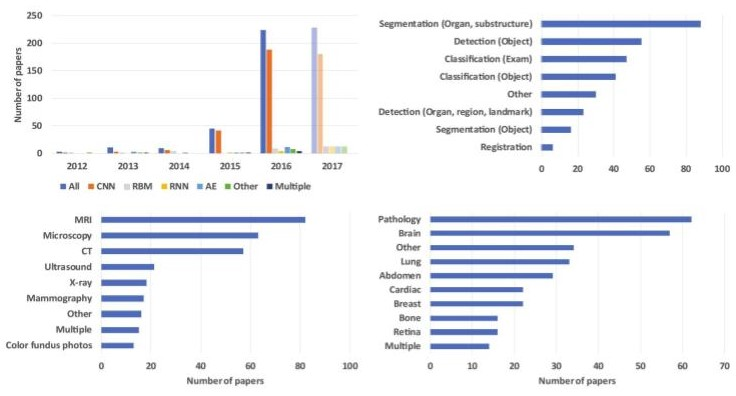
\includegraphics[width=1\textwidth]{figures/DL_CAD_statystyka.jpg}
	\caption{Statystyki dotyczące publikacji medycznych zawierających słowa kluczowe związane z głębokim uczeniem się.}
	\label{DL_CAD_stats}
\end{figure}

 Widoczny wzrost liczby publikacji nastąpił począwszy od 2015, co związane było z kilkuletnią adaptacją nowych metod w dziedzinie przetwarzania obrazów medycznych i gromadzeniem odpowiednich zbiorów danych. Lata 2016 i 2017 były pod pewnym względem przełomowe gdyż pojawiało się coraz więcej prac naukowych, w których przedstawiano rezultaty dokładności klasyfikacji na poziomie dorównującym ekspertom dziedzinowym.
 
 Dla przykładu, w Listopadzie 2016 ukazała się praca \cite{Gulshan2016} grupy Google Research z Mountain View w Kalifornii, gdzie zastosowano sieć GoogLeNet w wersji inception-v3 do zautomatyzowanej detekcji retinopatii cukrzycowej i cukrzycowego obrzęku plamki w obrazach dna oka. Wyniki porównano z panelem składającym się z 7 ekspertów, okulistów. Porównanie przedstawiono na Rys. \ref{CAD_opto}.
 \begin{figure}[h!]
 	\centering
 	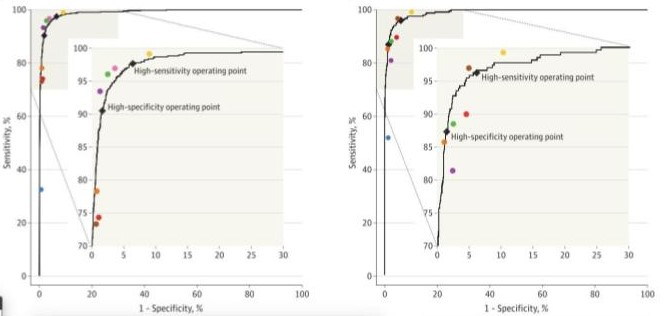
\includegraphics[width=0.7\textwidth]{figures/CAD-okulisci.jpg}
 	\caption{Porównanie automatycznej klasyfikacji retinopatii cukrzycowej i cukrzycowego obrzęku plamki z oceną panelu ekspertów.}
 	\label{CAD_opto}
 \end{figure}
 
 Na wykresach dla dwóch zadań klasyfikacyjnych umieszczono krzywe reprezentujące zależność swoistości od czułości dla algorytmu automatycznego oraz 7 punktów oznaczających wynik oceny każdego z okulistów. Ogółem mniej niż połowa ekspertów uzyskała lepszy wynik niż algorytm sztucznej inteligencji.
 
 Kolejna ciekawa praca tj. \cite{Esteva2017}, pojawiła się w czasopiśmie Nature w styczniu 2017 roku i traktowała o automatycznej detekcji nowotworów skóry na podstawie zdjęć. Autorzy wykorzystali dane składające się z 129.450 obrazów klinicznych, na których zobrazowano 2.032 różne schorzenia skóry. Ponownie do klasyfikacji wykorzystano sieć GoogleNet w wersji inception-v3. Wyniki klasyfikacji automatycznej porównano z oceną przeprowadzoną przez 21 certyfikowanych dermatologów. Przykład porównania zaprezentowano na Rys. \ref{CAD_derma}. 
 
 \begin{figure}[h!]
 	\centering
 	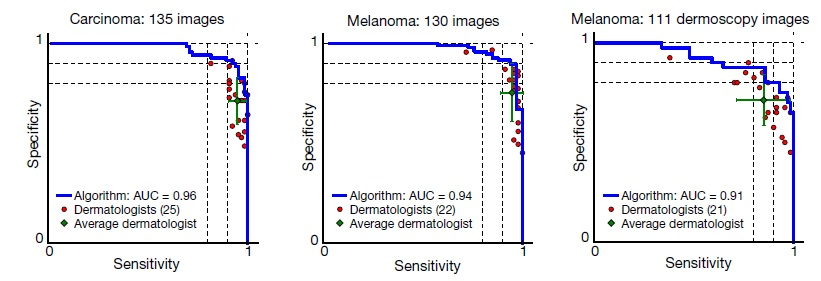
\includegraphics[width=0.9\textwidth]{figures/CAD-dermatolodzy.jpg}
 	\caption{Porównanie automatycznej klasyfikacji 3 chorób skóry z oceną ekspertów dermatologów.}
 	\label{CAD_derma}
 \end{figure}

Wykres przedstawia zależność czułości od swoistości. Czerwonymi punktami oznaczono wynik oceny poszczególnych ekspertów, a zielonym krzyżykiem wynik uśredniony. W każdym przypadku średnia ocena była gorsza od automatycznej klasyfikacji.

Obrazy medyczne nie są jedynymi danymi, które z powodzeniem są przetwarzane za pomocą metod głębokiego uczenia się. W lipcu 2017, przez grupę ze Stanford University została opublikowana praca \cite{2017arXiv170701836R} dotycząca klasyfikacji arytmii na podstawie szeregów czasowych zapisanych na elektrokardiogramach. Autorzy wykorzystali dane z 64.121 elektrokardiogramów, próbkowanych z częstotliwością 200 Hz, pochodzących od 29.163 pacjentów. Zaprojektowano dedykowaną, 34-warstwową sieć konwolucyjną do detekcji 12 różnych dysfunkcji pracy serca, pracy prawidłowej i szumów (łącznie 14 klas). Wyniki klasyfikacji porównano z oceną prowadzoną przez 3 kardiologów. Średnia dokładność z oceny automatycznej wyniosła 80\%, natomiast manualnej 72\%.

Podobnych przykładów zostało opublikowanych dużo więcej. Architektura AlexNet z sukcesem była użyta do detekcji polipów w kolonoskopii w \cite{Tajbakhsh2016}. Sieć ResNet sprawdziła się w badaniach zrealizowanych w \cite{Erickson2018} w Mayo Clinic Rotschester. Dotyczyły one radio-genomiki i rozróżnienia zmian w mózgu bez konieczności biopsji. Złożenia natomiast z sukcesem zaaplikowano w pracach dotyczących detekcji nowotworów płuc, gdzie modele bazowe analizowały różne skale problemu (zob. \cite{LungChalenge}). W wielu pracach dotyczących radiologii raportuje się dokładność klasyfikacji automatycznej znacząco przewyższające możliwości dziedzinowych ekspertów np. \cite{Christiansen2018, Sarraf2016, Glasser2016, 2016arXiv160605718W}.

Powyższe przykłady pokazują, że dla szczególnych przypadków pewien element pracy eksperta zajmującego się danymi medycznymi (np. radiologa) może być z sukcesem wspomagany (lub nawet zastąpiony) przez algorytmy głębokiego uczenia się. Fakt ten ma swoje odzwierciedlenie w liczbie nowych firm stosujących głębokie sieci neuronowe do wspomagania medycyny i uzyskujących certyfikację medyczną. Infografikę przedstawiającą dynamikę tych zmian zaprezentowano na Rys. \ref{fda_cert}.

\begin{figure}[h!]
	\centering
	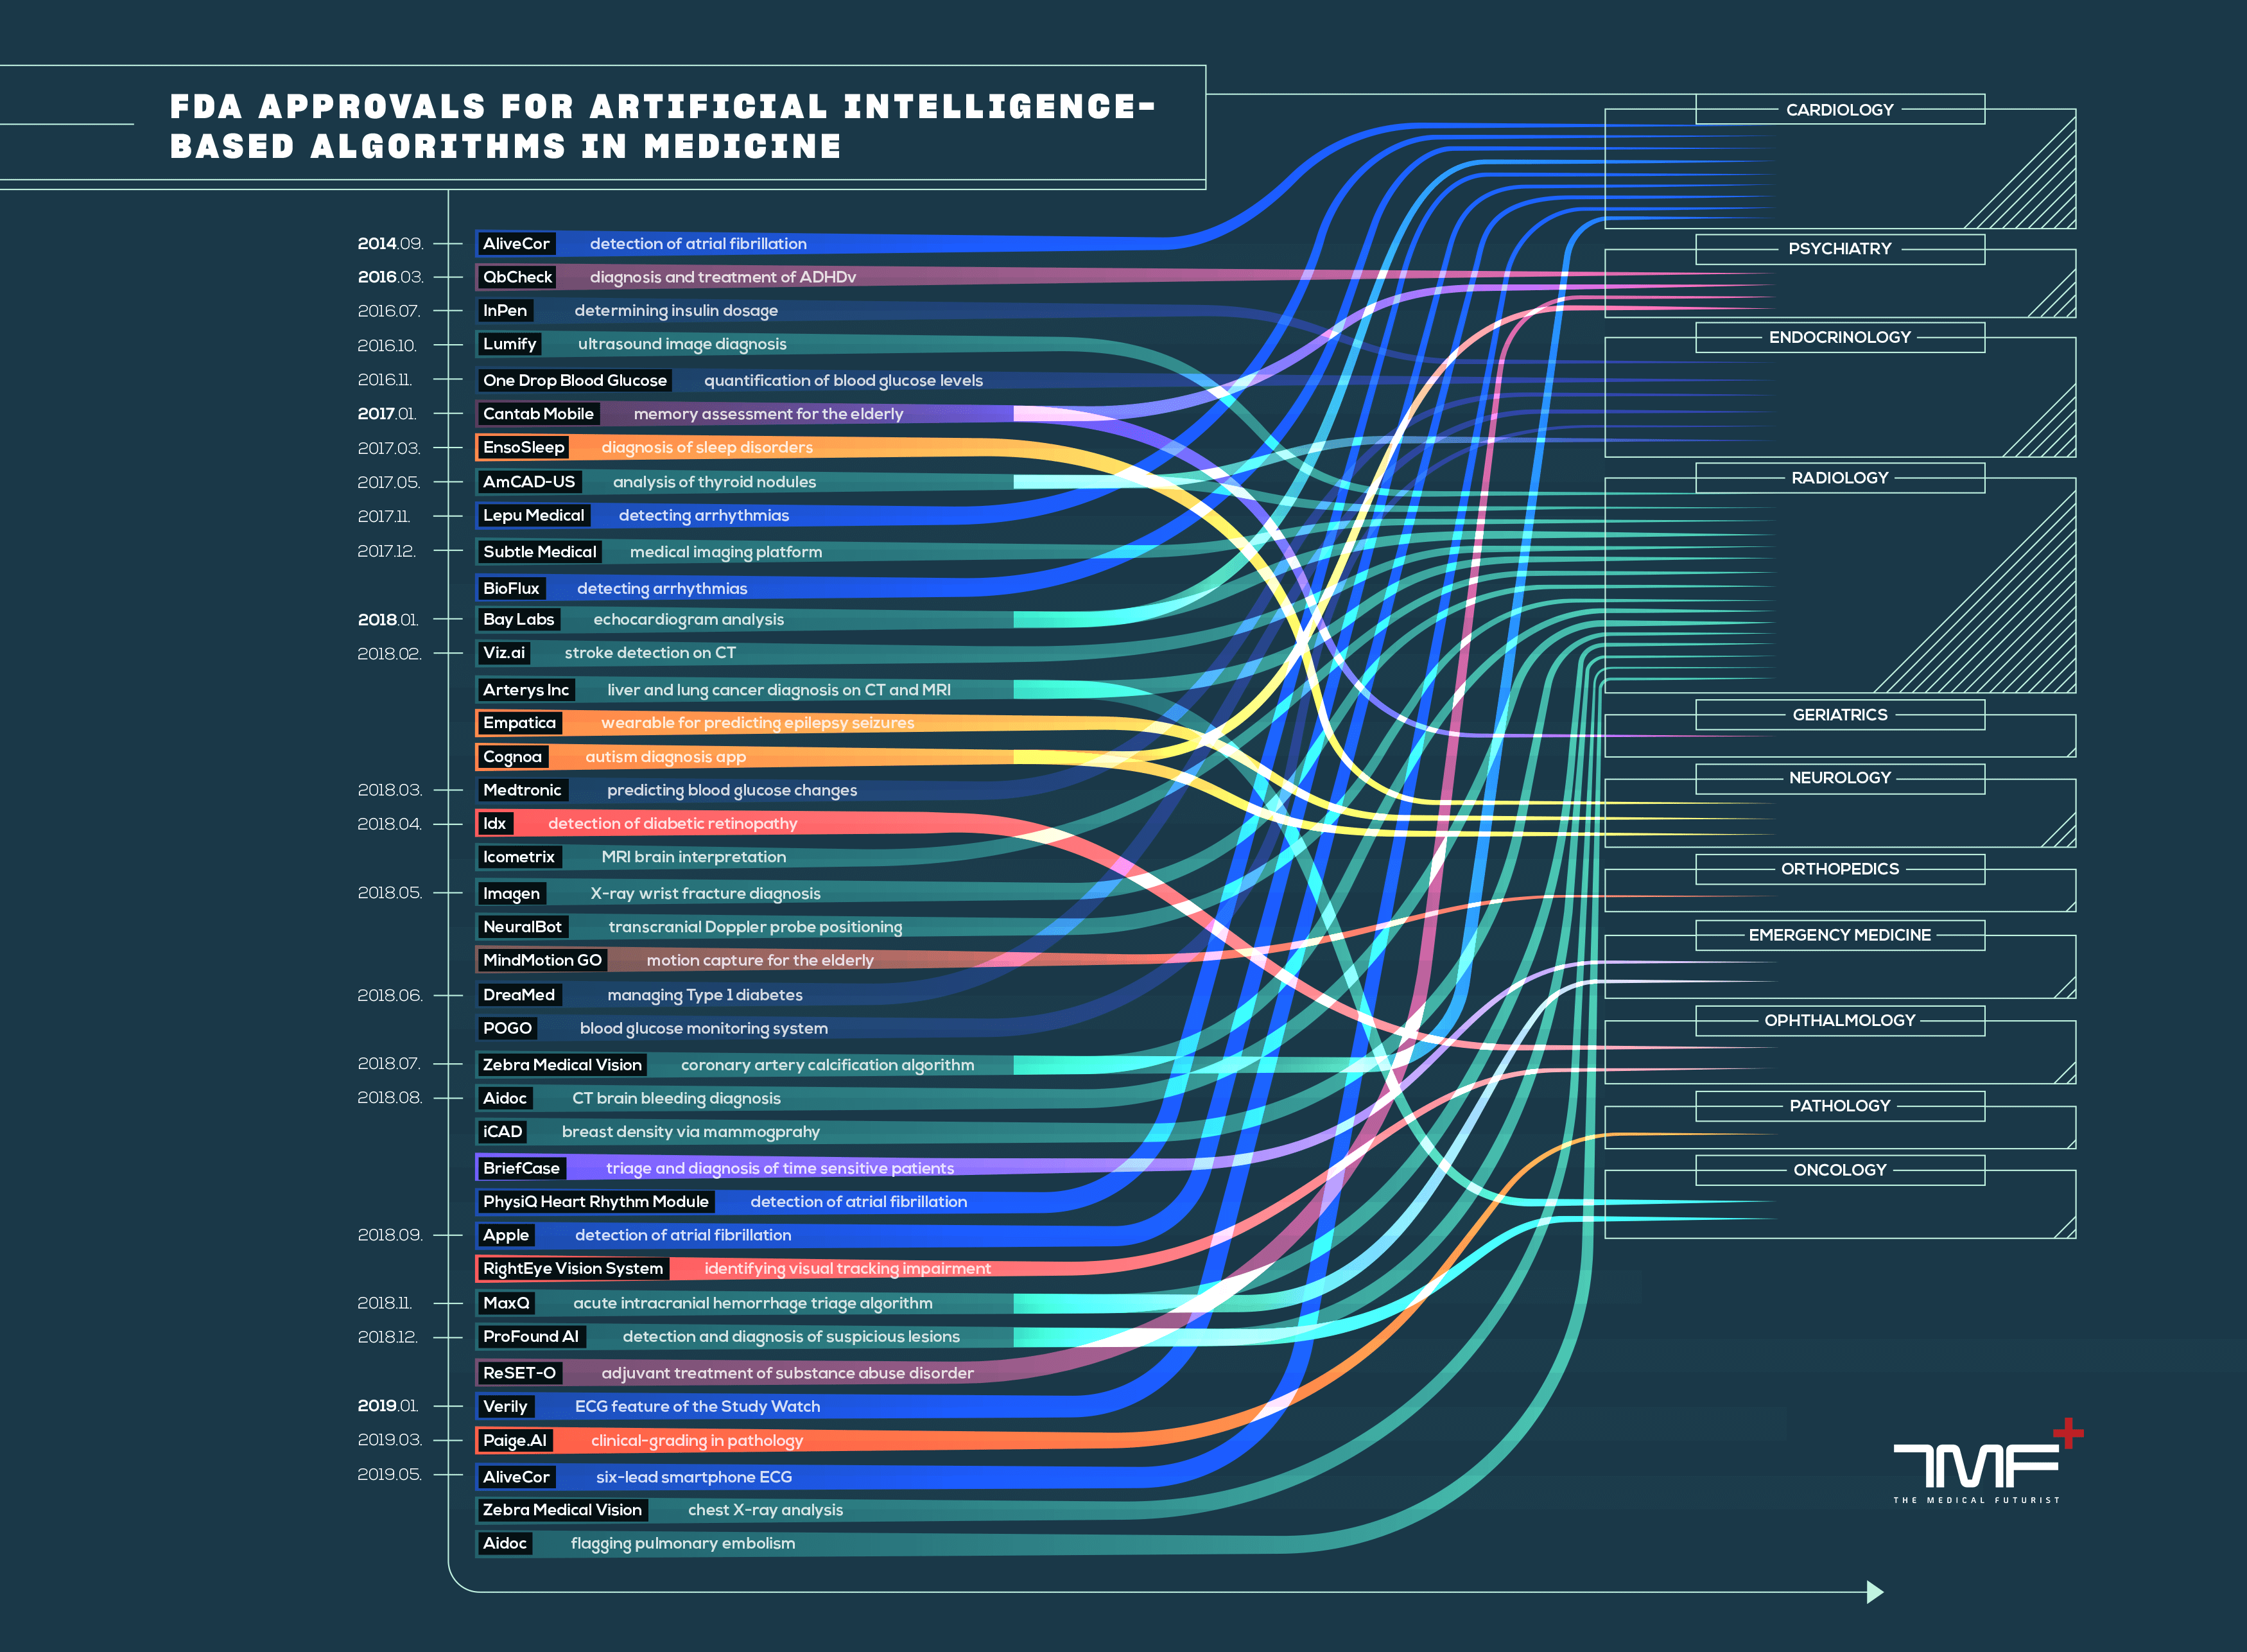
\includegraphics[width=0.9\textwidth]{figures/fda_for_ai.png}
	\caption{Firmy stosujące w swoich produktach głębokie sieci neuronowe, uzyskujące certyfikację FDA.}
	\label{fda_cert}
\end{figure}

Należy jednak podkreślić, że jest również szereg problemów wiążących się z wykorzystaniem tego rodzaju sztucznej inteligencji w medycynie. Do najważniejszych należą:
\begin{enumerate}
	\item Gromadzenie dużych zbiorów danych z odpowiednimi etykietami.
	\item Wykorzystanie heterogenicznych danych pochodzących np. z wielu urządzeń lub modalności.
	\item Kalibracja i szacowanie niepewności wyników modeli.
	\item Unifikacja modeli wykonujących podobne zadania.
	\item Minimalizacja liczby parametrów modelu przy zachowaniu satysfakcjonującego poziomu dokładności.
\end{enumerate}
Więcej na temat ograniczeń metod głębokiego uczenia się można przeczytać również w \cite{Marcus2018}.

Dyskusja dotycząca tych problemów wciąż jest tematem wielu paneli dyskusyjnych i debat konferencyjnych (zob np. \cite{NVIDIApanel}). Najbardziej zaawansowane prace dotyczą problemu gromadzenia dużych zbiorów danych medycznych, co wymaga bliskiej współpracy ekspertów medycznych z ekspertami od uczenia maszynowego. Często konieczna jest również modyfikacja bądź tworzenie dedykowanych programów do akwizycji danych medycznych. Jako przykłady takich inicjatyw można wymienić programy Stanford Medicine \cite{MedicalImageNet}, Harvard School of Medicine \cite{HMS} czy Massachusetts General Hospital, które w swoich repozytoriach zgromadziły już dziesiątki milionów zdjęć radiologicznych (za \cite{MGH}). Ponadto w roku 2018, na konferencji NVIDIA GTC (GPU Technology Conference) w San Jose (Kalifornia), Amerykańskie Stowarzyszenie Radiologii i stowarzyszenie MICCAI (od ang. \textit{Medical Image Computing and Computer Assisted Intervention}) ogłosiły porozumienie, co do wspólnej współpracy mającej na celu eliminacje barier legislacyjnych związanych ze współpracą przy pozyskiwaniu danych i wykorzystania algorytmów uczenia maszynowego.

Autor tej rozprawy jest świadom ograniczeń jakie są związane z wykorzystaniem algorytmów głębokiego uczenia się. Jednocześnie jednak nowe metody i ostatnie sukcesy zastosowań współczesnych sztucznych sieci neuronowych w aplikacjach medycznych stanowią silną motywację do przeprowadzenia własnych badań z ich wykorzystaniem.


    
